\documentclass[portrait,final,a0paper,fontscale=0.277]{baposter}

\usepackage{calc}
\usepackage{graphicx}
\usepackage{amsmath}
\usepackage{amssymb}
\usepackage{relsize}
\usepackage{multirow}
\usepackage{rotating}
\usepackage{bm}
\usepackage{enumitem}
\usepackage{url}
\usepackage{booktabs}

\usepackage{graphicx}
\usepackage{multicol}

%\usepackage{times}
%\usepackage{helvet}
%\usepackage{bookman}
\usepackage{palatino}

\newcommand{\captionfont}{\footnotesize}

\graphicspath{{images/}{../images/}}
\usetikzlibrary{calc}


\newcommand{\Matrix}[1]{\begin{bmatrix} #1 \end{bmatrix}}
\newcommand{\Vector}[1]{\begin{pmatrix} #1 \end{pmatrix}}

\newcommand*{\norm}[1]{\mathopen\| #1 \mathclose\|}% use instead of $\|x\|$
\newcommand*{\abs}[1]{\mathopen| #1 \mathclose|}% use instead of $\|x\|$
\newcommand*{\normLR}[1]{\left\| #1 \right\|}% use instead of $\|x\|$

\newcommand*{\SET}[1]  {\ensuremath{\mathcal{#1}}}
\newcommand*{\FUN}[1]  {\ensuremath{\mathcal{#1}}}
\newcommand*{\MAT}[1]  {\ensuremath{\boldsymbol{#1}}}
\newcommand*{\VEC}[1]  {\ensuremath{\boldsymbol{#1}}}
\newcommand*{\CONST}[1]{\ensuremath{\mathit{#1}}}

\DeclareMathOperator*{\argmax}{arg\,max}
\DeclareMathOperator*{\diag}{diag}
\DeclareMathOperator*{\argmin}{arg\,min}
\DeclareMathOperator*{\vectorize}{vec}
\DeclareMathOperator*{\reshape}{reshape}

%\font\dsfnt=dsrom12

\newcommand{\SNN}{\ensuremath{\mathbb N}}
\newcommand{\SRR}{\ensuremath{\mathbb R}}
\newcommand{\SZZ}{\ensuremath{\mathbb Z}}
%-----------------------------------------------------------------------------
% Matrices of the shape model
\renewcommand{\a}{\VEC\alpha}
\renewcommand{\v}{\VEC v}
\renewcommand{\l}{\VEC l}
\newcommand*{\m}{\VEC{\mu}}
\newcommand*{\M}{\MAT{M}}
\renewcommand*{\P}{\MAT{\Pi}}

%\newcommand{\J}{\SET J}
\newcommand{\J}{\SET{P}}
\newcommand{\Active}{\mathcal{A}}
\newcommand{\Selection}{\mathbf{S}}
\newcommand{\AllSelections}{\mathfrak{S}}
\newcommand{\Params}{\VEC\Theta}

%%%%%%%%%%%%%%%%%%%%%%%%%%%%%%%%%%%%%%%%%%%%%%%%%%%%%%%%%%%%%%%%%%%%%%%%%%%%%%%%
%%%% Some math symbols used in the text
%%%%%%%%%%%%%%%%%%%%%%%%%%%%%%%%%%%%%%%%%%%%%%%%%%%%%%%%%%%%%%%%%%%%%%%%%%%%%%%%

%%%%%%%%%%%%%%%%%%%%%%%%%%%%%%%%%%%%%%%%%%%%%%%%%%%%%%%%%%%%%%%%%%%%%%%%%%%%%%%%
% Multicol Settings
%%%%%%%%%%%%%%%%%%%%%%%%%%%%%%%%%%%%%%%%%%%%%%%%%%%%%%%%%%%%%%%%%%%%%%%%%%%%%%%%
\setlength{\columnsep}{1.5em}
\setlength{\columnseprule}{0mm}

%%%%%%%%%%%%%%%%%%%%%%%%%%%%%%%%%%%%%%%%%%%%%%%%%%%%%%%%%%%%%%%%%%%%%%%%%%%%%%%%
% Save space in lists. Use this after the opening of the list
%%%%%%%%%%%%%%%%%%%%%%%%%%%%%%%%%%%%%%%%%%%%%%%%%%%%%%%%%%%%%%%%%%%%%%%%%%%%%%%%
\newcommand{\compresslist}{%
\setlength{\itemsep}{1pt}%
\setlength{\parskip}{0pt}%
\setlength{\parsep}{0pt}%
}

%%%%%%%%%%%%%%%%%%%%%%%%%%%%%%%%%%%%%%%%%%%%%%%%%%%%%%%%%%%%%%%%%%%%%%%%%%%%%%
%%% Begin of Document
%%%%%%%%%%%%%%%%%%%%%%%%%%%%%%%%%%%%%%%%%%%%%%%%%%%%%%%%%%%%%%%%%%%%%%%%%%%%%%

\begin{document}

%%%%%%%%%%%%%%%%%%%%%%%%%%%%%%%%%%%%%%%%%%%%%%%%%%%%%%%%%%%%%%%%%%%%%%%%%%%%%%
%%% Here starts the poster
%%%---------------------------------------------------------------------------
%%% Format it to your taste with the options
%%%%%%%%%%%%%%%%%%%%%%%%%%%%%%%%%%%%%%%%%%%%%%%%%%%%%%%%%%%%%%%%%%%%%%%%%%%%%%
% Define some colors

\definecolor{lightorange}{rgb}{0.9,0.4,0}
\definecolor{lightestorange}{rgb}{1,0.8,0.5}
\definecolor{darkorange}{rgb}{0.2,0.1,0}

\hyphenation{resolution occlusions}
%%
\begin{poster}%
  % Poster Options
  {
  % Show grid to help with alignment
  grid=false,
  % Column spacing
  colspacing=1em,
  % Color style
  bgColorOne=lightestorange,
  bgColorTwo=white,
  borderColor=darkorange,
  headerColorOne=darkorange,
  headerColorTwo=lightorange,
  headerFontColor=white,
  boxColorOne=lightestorange,
  boxColorTwo=lightorange,
  % Format of textbox
  textborder=faded,
  % Format of text header
  eyecatcher=true,
  headerborder=closed,
  headerheight=0.1\textheight,
%  textfont=\sc, An example of changing the text font
  headershape=roundedright,
  headershade=shadelr,
  headerfont=\Large\bf\textsc, %Sans Serif
  textfont={\setlength{\parindent}{1.5em}},
  boxshade=plain,
%  background=shade-tb,
  background=plain,
  linewidth=2pt
  }
  % Eye Catcher
  {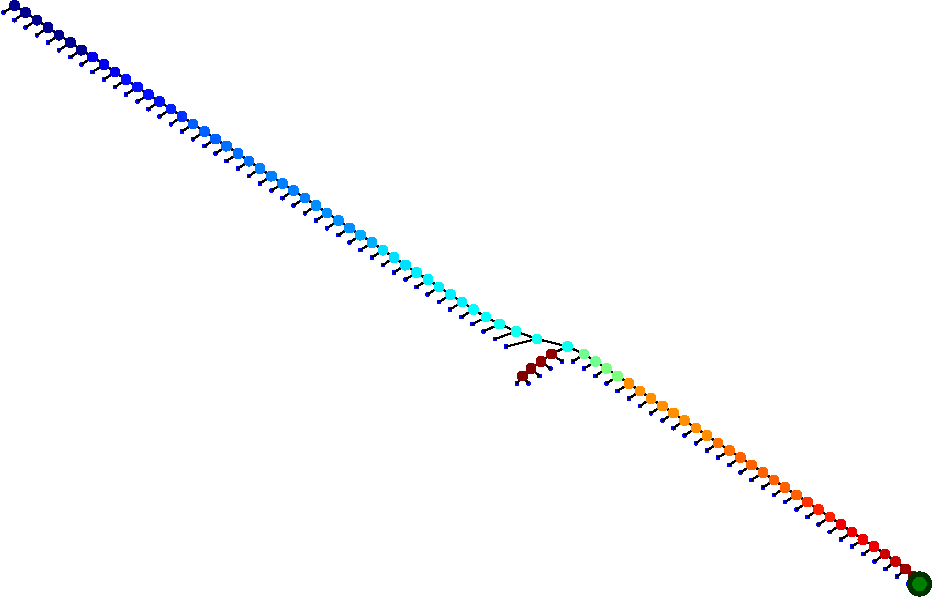
\includegraphics[height=7em]{images/search_tree_ex1-crop.pdf}} 
  % Title
  {\bf\textsc{Optimal Landmark Detection using Shape Models and Branch and Bound}\vspace{0.5em}}
  % Authors
  {\textsc{\{ Brian.Amberg and Thomas.Vetter \}@unibas.ch}}
  % University logo
  {% The makebox allows the title to flow into the logo, this is a hack because of the L shaped logo.
    
\includegraphics[height=9.0em]{images/logo}
  }

%%%%%%%%%%%%%%%%%%%%%%%%%%%%%%%%%%%%%%%%%%%%%%%%%%%%%%%%%%%%%%%%%%%%%%%%%%%%%%
%%% Now define the boxes that make up the poster
%%%---------------------------------------------------------------------------
%%% Each box has a name and can be placed absolutely or relatively.
%%% The only inconvenience is that you can only specify a relative position 
%%% towards an already declared box. So if you have a box attached to the 
%%% bottom, one to the top and a third one which should be in between, you 
%%% have to specify the top and bottom boxes before you specify the middle 
%%% box.
%%%%%%%%%%%%%%%%%%%%%%%%%%%%%%%%%%%%%%%%%%%%%%%%%%%%%%%%%%%%%%%%%%%%%%%%%%%%%%
    %
    % A coloured circle useful as a bullet with an adjustably strong filling
    \newcommand{\colouredcircle}{%
      \tikz{\useasboundingbox (-0.2em,-0.32em) rectangle(0.2em,0.32em); \draw[draw=black,fill=lightblue,line width=0.03em] (0,0) circle(0.18em);}}

%%%%%%%%%%%%%%%%%%%%%%%%%%%%%%%%%%%%%%%%%%%%%%%%%%%%%%%%%%%%%%%%%%%%%%%%%%%%%%
  \headerbox{Problem}{name=problem,column=0,row=0}{
%%%%%%%%%%%%%%%%%%%%%%%%%%%%%%%%%%%%%%%%%%%%%%%%%%%%%%%%%%%%%%%%%%%%%%%%%%%%%%
  Fitting statistical 2D and 3D shape models to images is necessary for a
  variety of tasks, such as video editing and face recognition. Much progress
  has been made on local fitting from an initial guess, but determining a close
  enough initial guess is still an open problem. We propose a method to locate
  fiducial points, which can then be used to initialize the fitting.
 }

%%%%%%%%%%%%%%%%%%%%%%%%%%%%%%%%%%%%%%%%%%%%%%%%%%%%%%%%%%%%%%%%%%%%%%%%%%%%%%
  \headerbox{Contributions}{name=contribution,column=0,below=problem}{
%%%%%%%%%%%%%%%%%%%%%%%%%%%%%%%%%%%%%%%%%%%%%%%%%%%%%%%%%%%%%%%%%%%%%%%%%%%%%%
  We overcome the inherent ambiguity in landmark detection by using global shape
  information. We solve the  combinatorial problem of selecting out of a large
  number of candidate landmark detections the configuration which is best
  supported by a shape model. Our method, as opposed to previous approaches,
  always finds the globally optimal configuration.

  The algorithm can be applied to a very general class of shape models and is
  independent of the underlying feature point detector. Its theoretic optimality
  is shown, and it is evaluated on a large face dataset.
  }

%%%%%%%%%%%%%%%%%%%%%%%%%%%%%%%%%%%%%%%%%%%%%%%%%%%%%%%%%%%%%%%%%%%%%%%%%%%%%%
\headerbox{Results}{name=results,column=1,span=2,row=0}{
  %%%%%%%%%%%%%%%%%%%%%%%%%%%%%%%%%%%%%%%%%%%%%%%%%%%%%%%%%%%%%%%%%%%%%%%%%%%%%%
  {
\smaller\centering
\begin{tabular}{@{}rccccccc@{}}
\begin{sideways}\makebox[0pt][c]{Success}\end{sideways} &
\parbox[c]{0.11\linewidth}{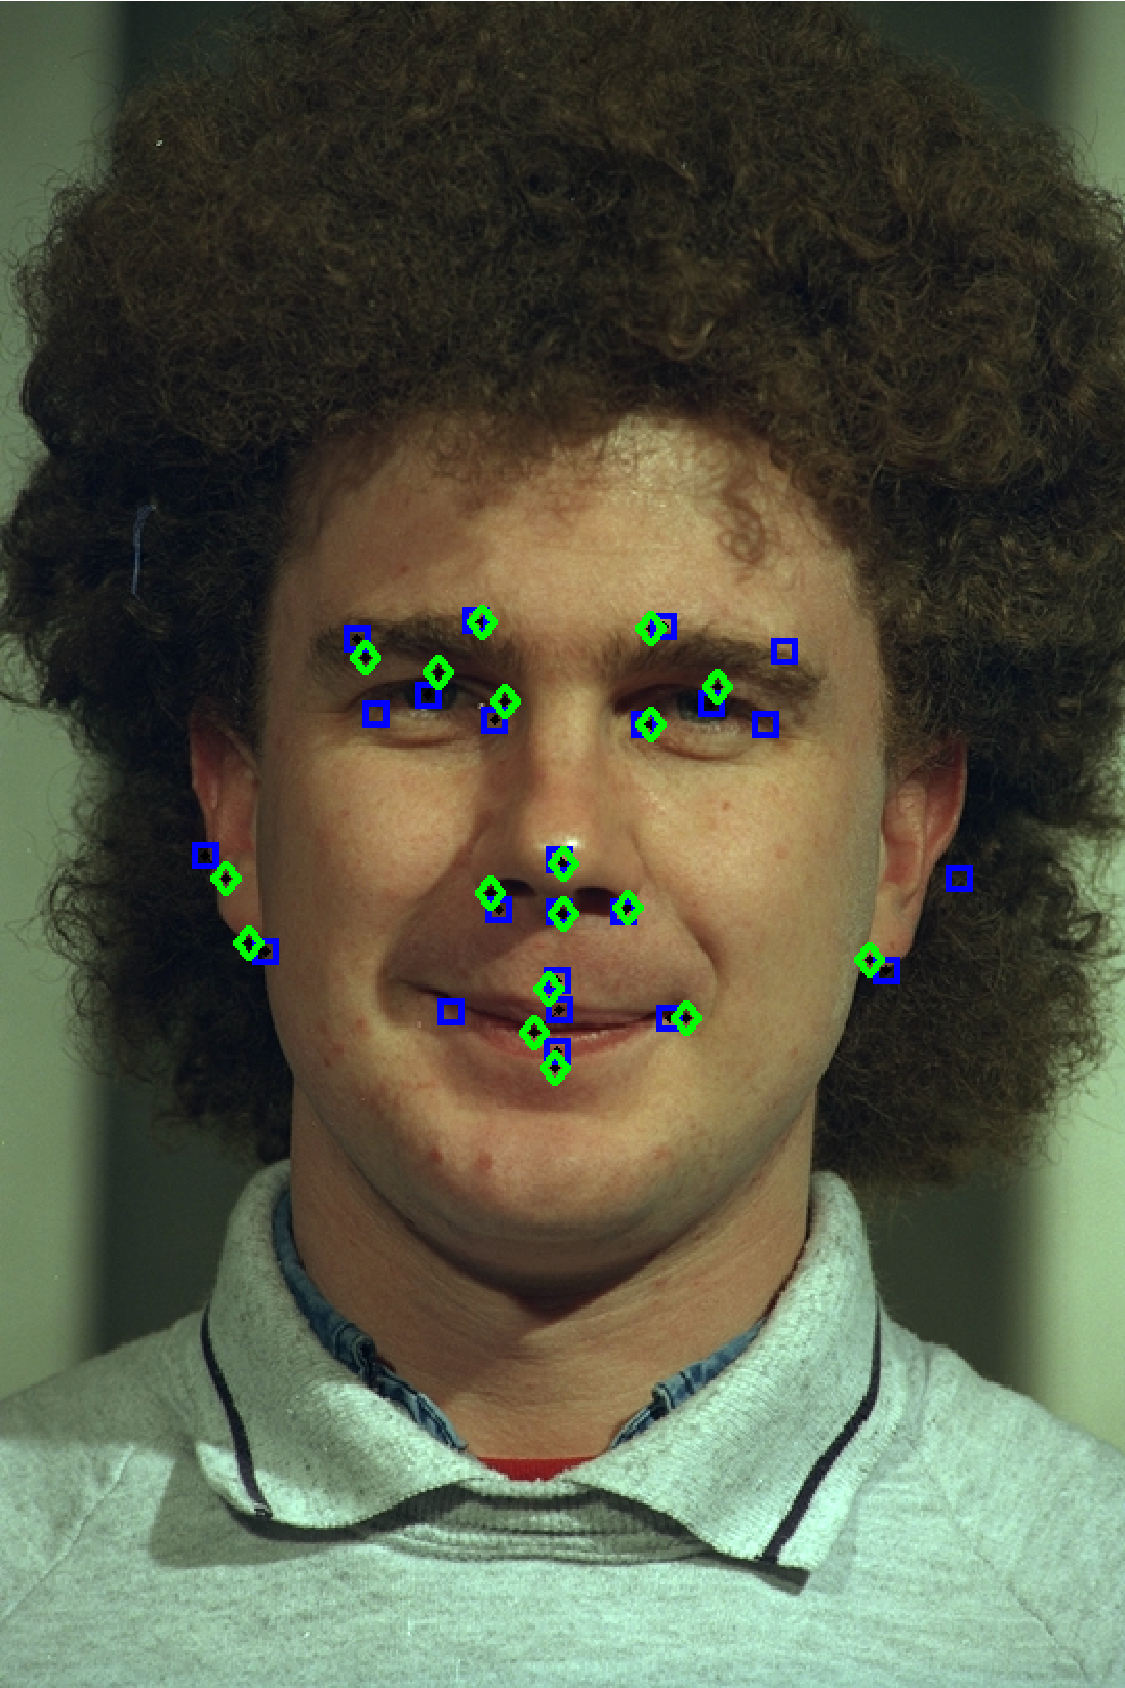
\includegraphics[width=\linewidth]{images/l_fa_success_1.pdf}} &
\parbox[c]{0.11\linewidth}{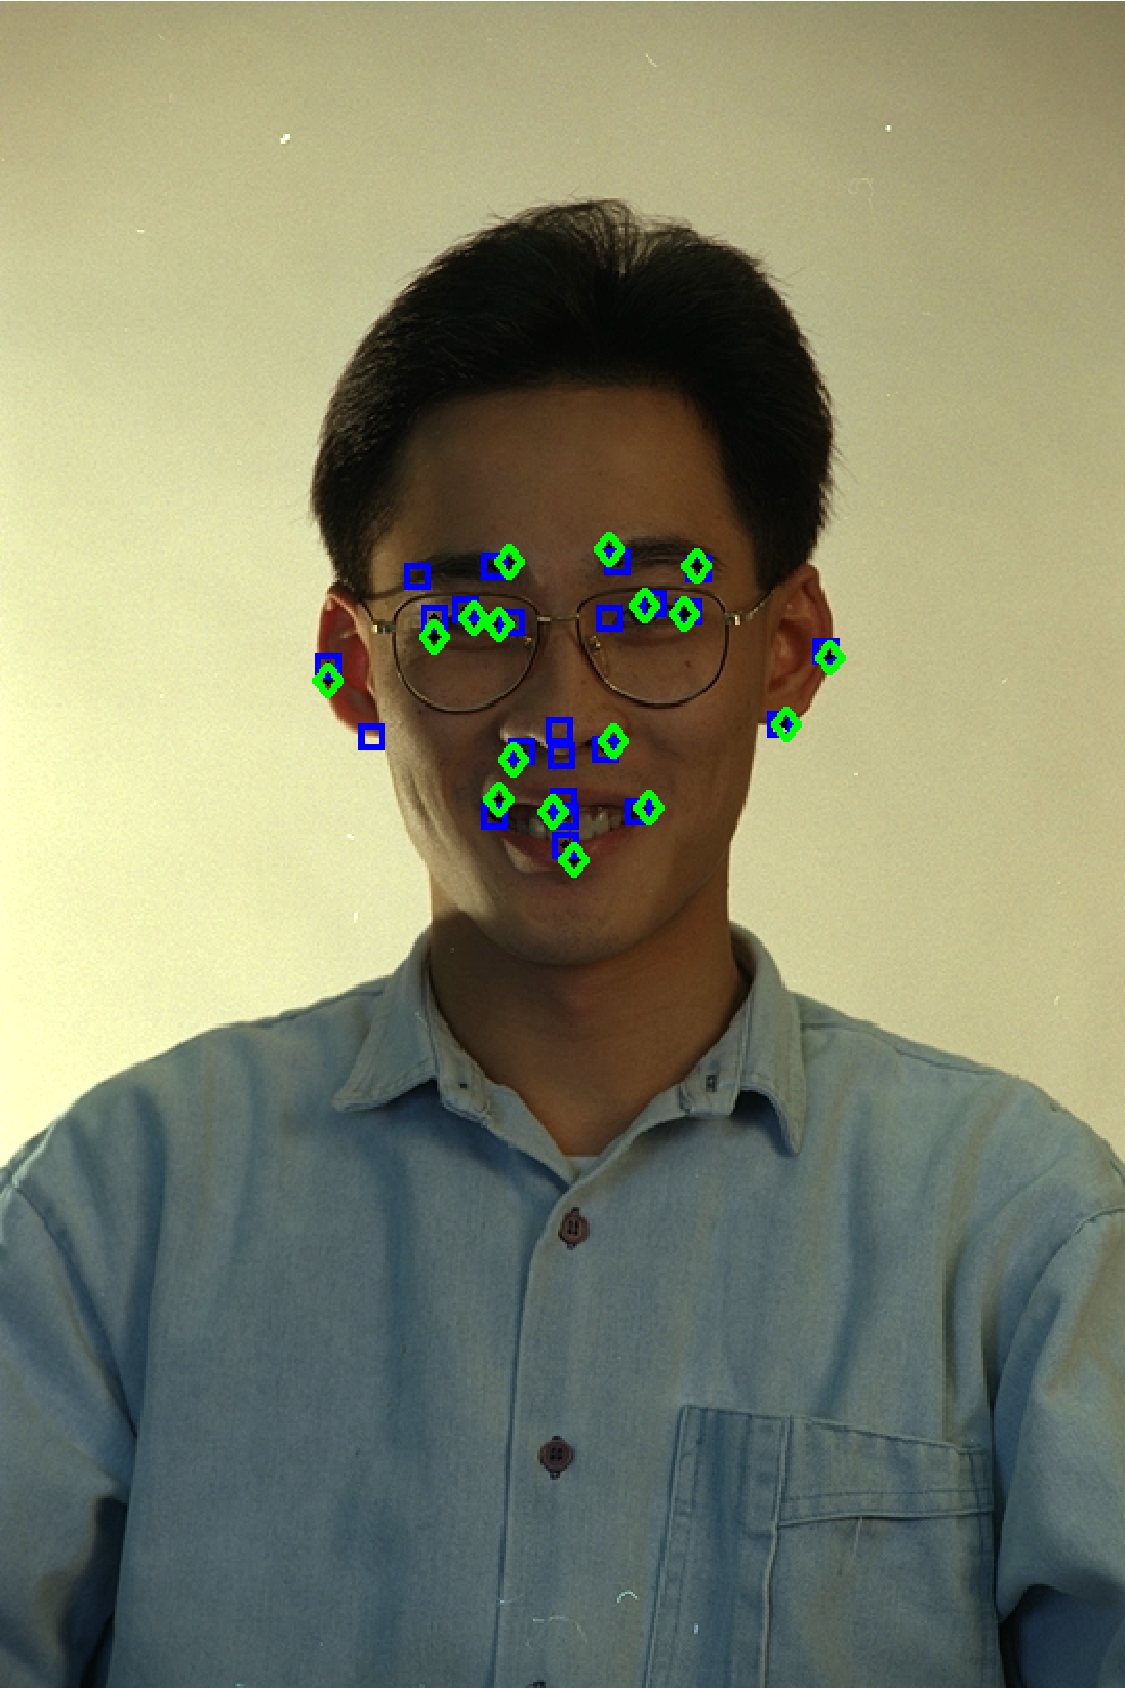
\includegraphics[width=\linewidth]{images/l_fb_success_1.pdf}} &
\parbox[c]{0.11\linewidth}{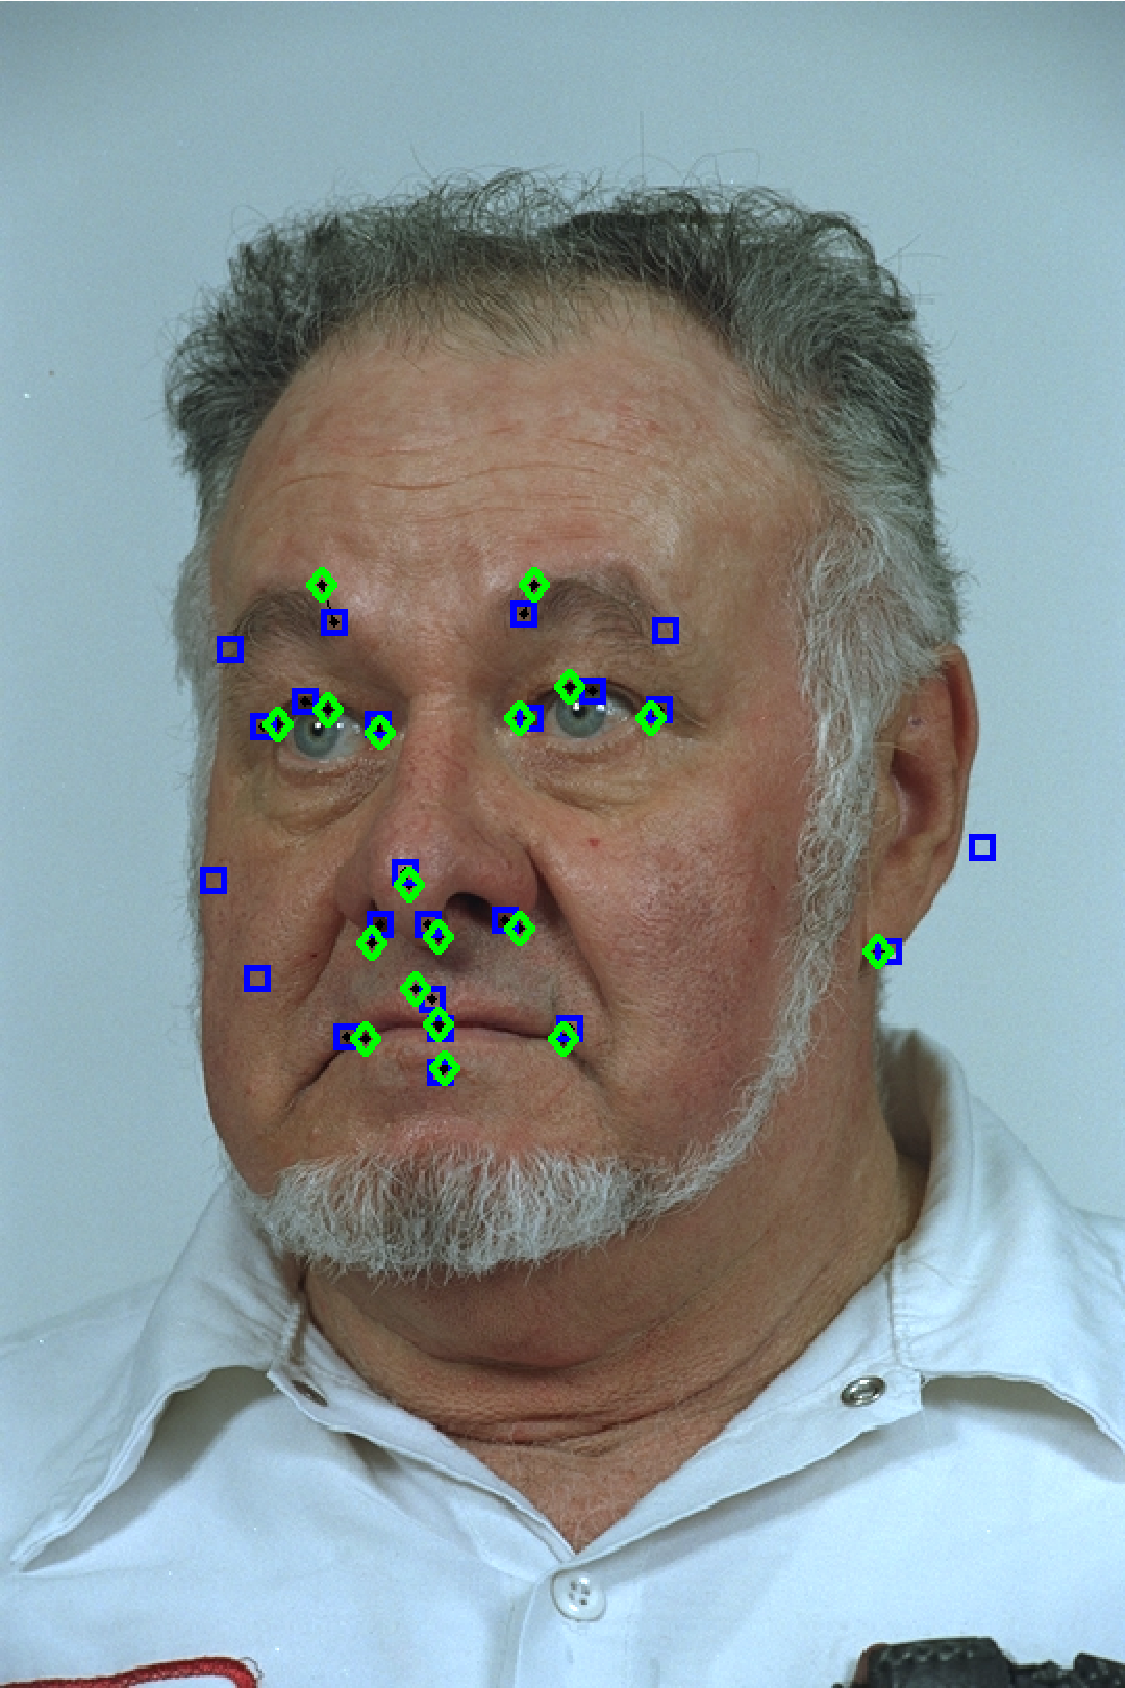
\includegraphics[width=\linewidth]{images/l_ql_success_1.pdf}} &
\parbox[c]{0.11\linewidth}{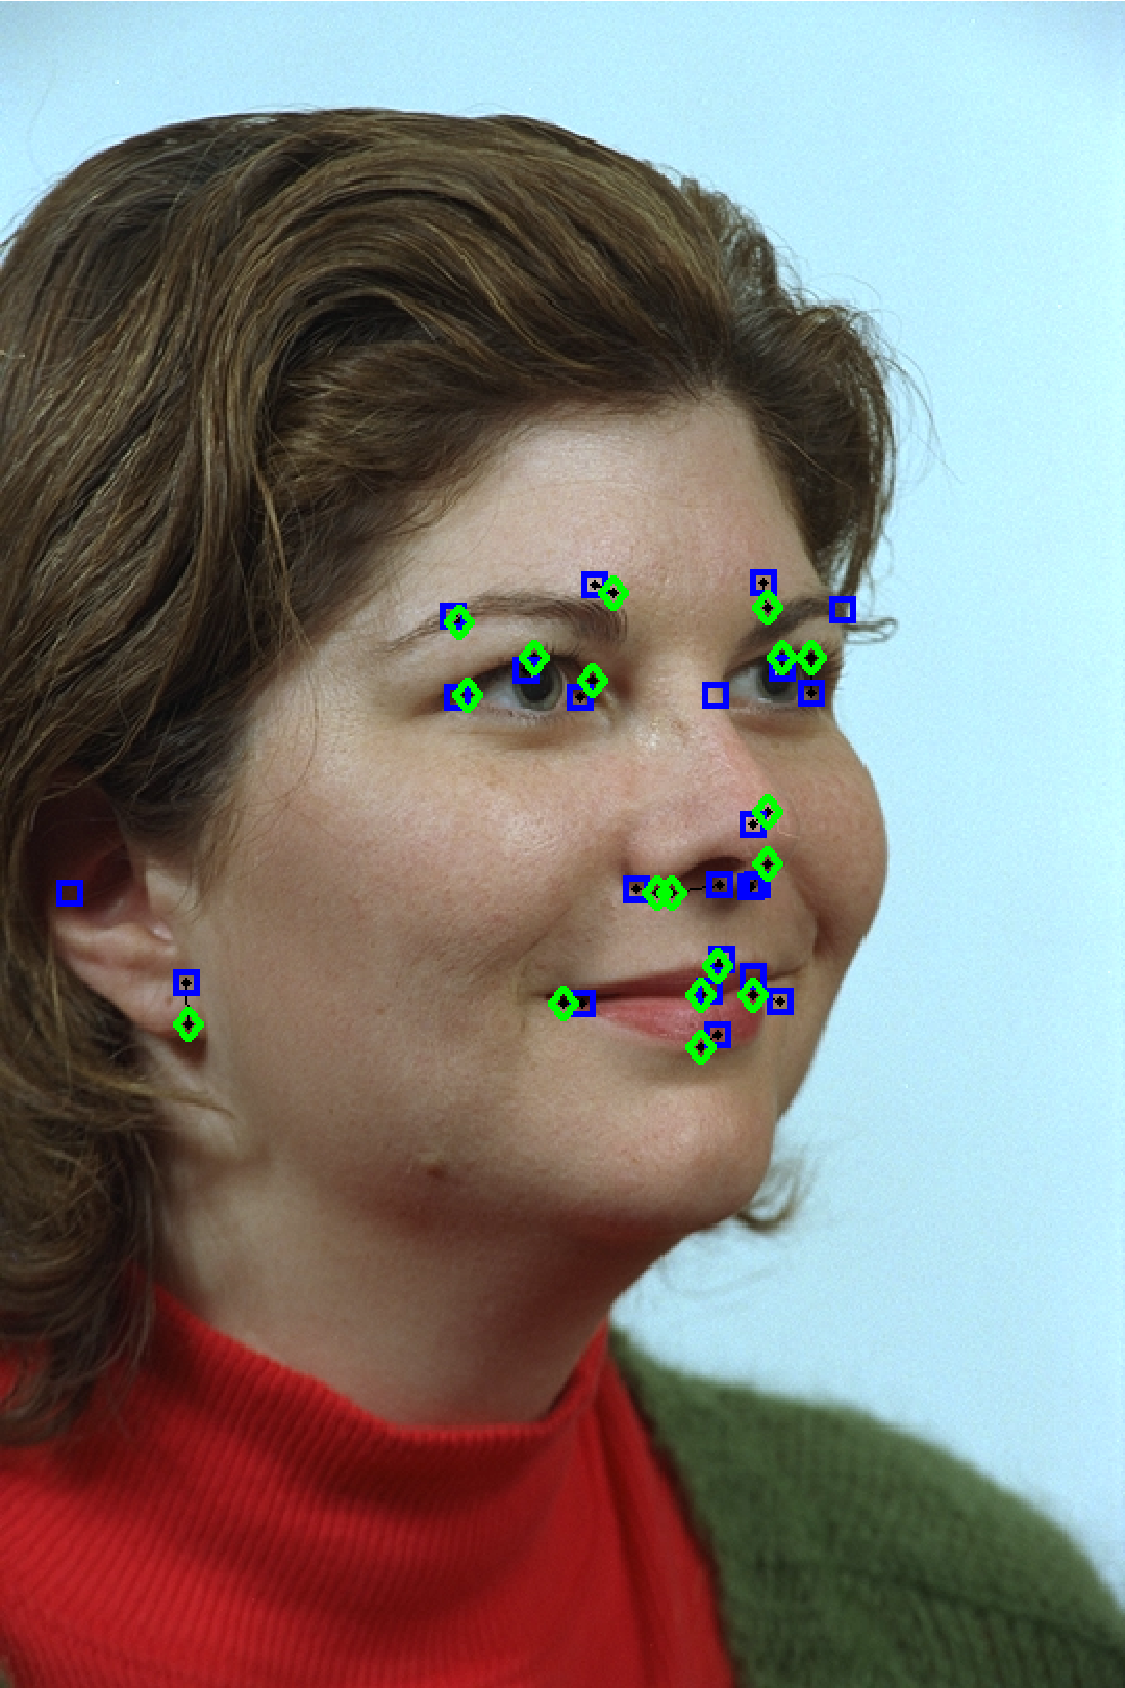
\includegraphics[width=\linewidth]{images/l_qr_success_1.pdf}} &
\parbox[c]{0.11\linewidth}{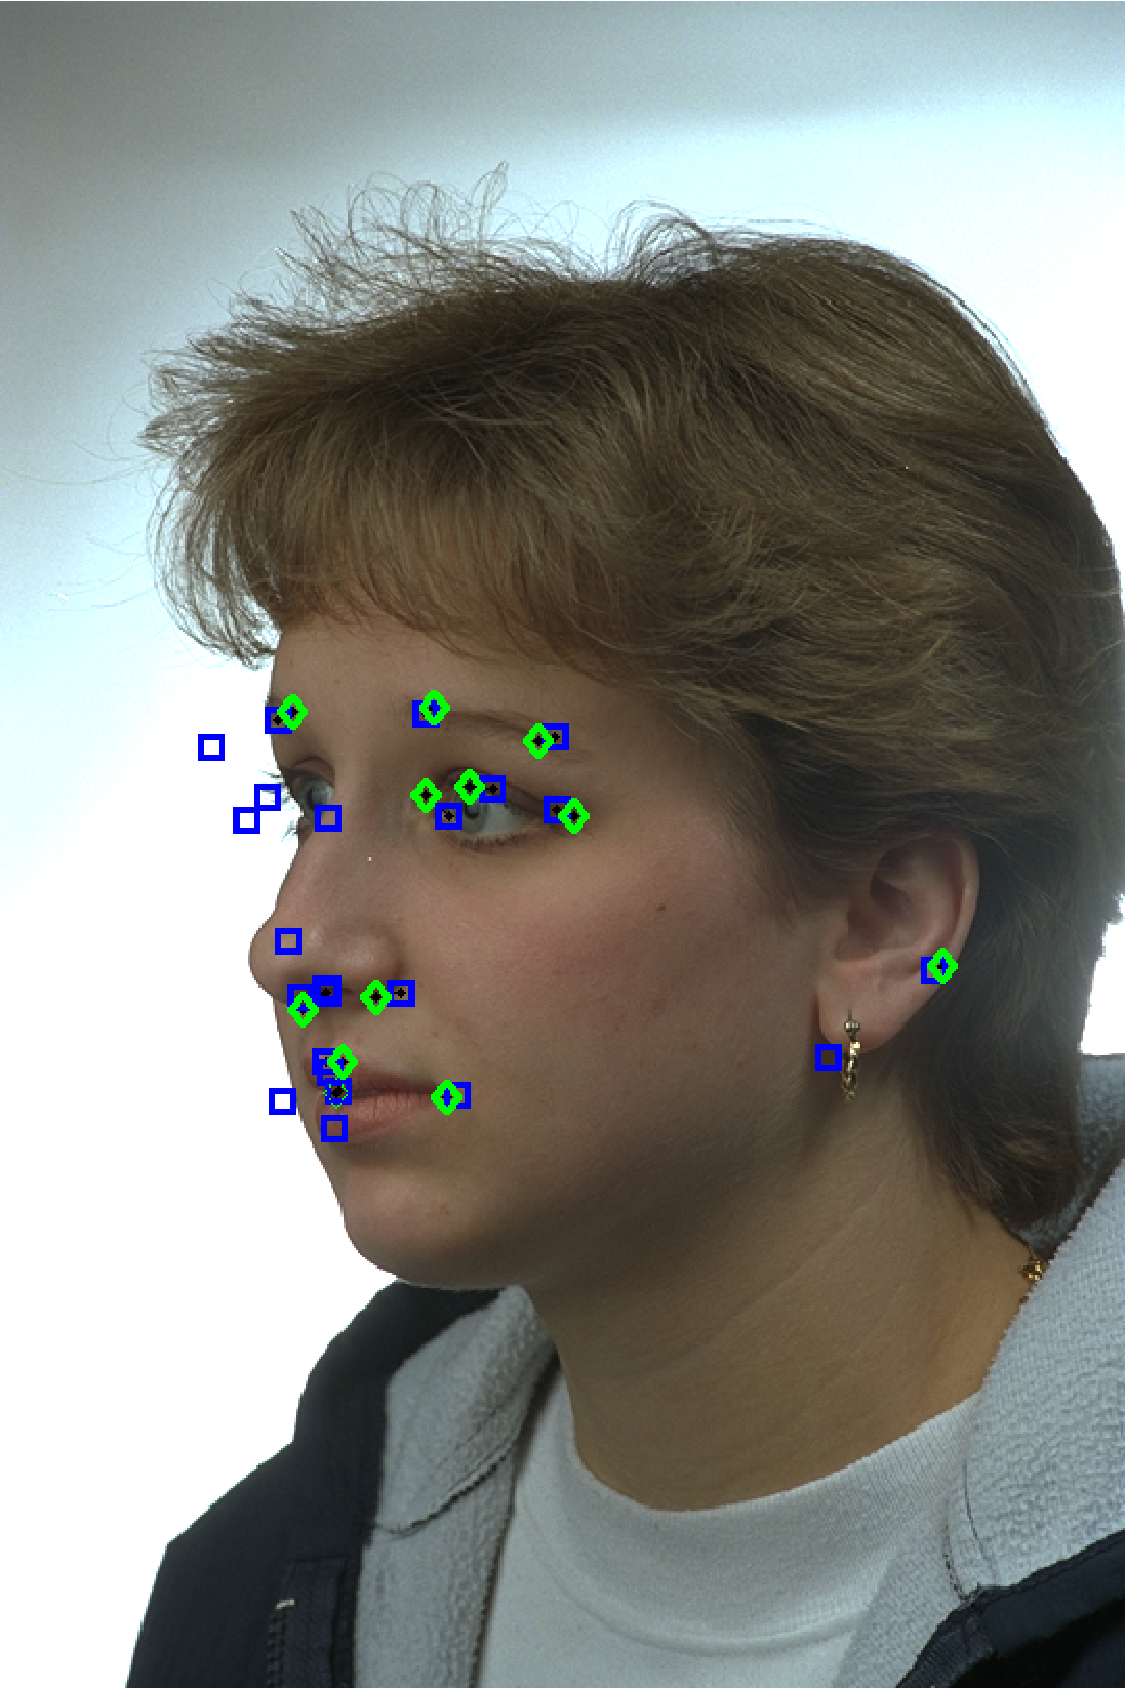
\includegraphics[width=\linewidth]{images/l_hl_success_1.pdf}} &
\parbox[c]{0.11\linewidth}{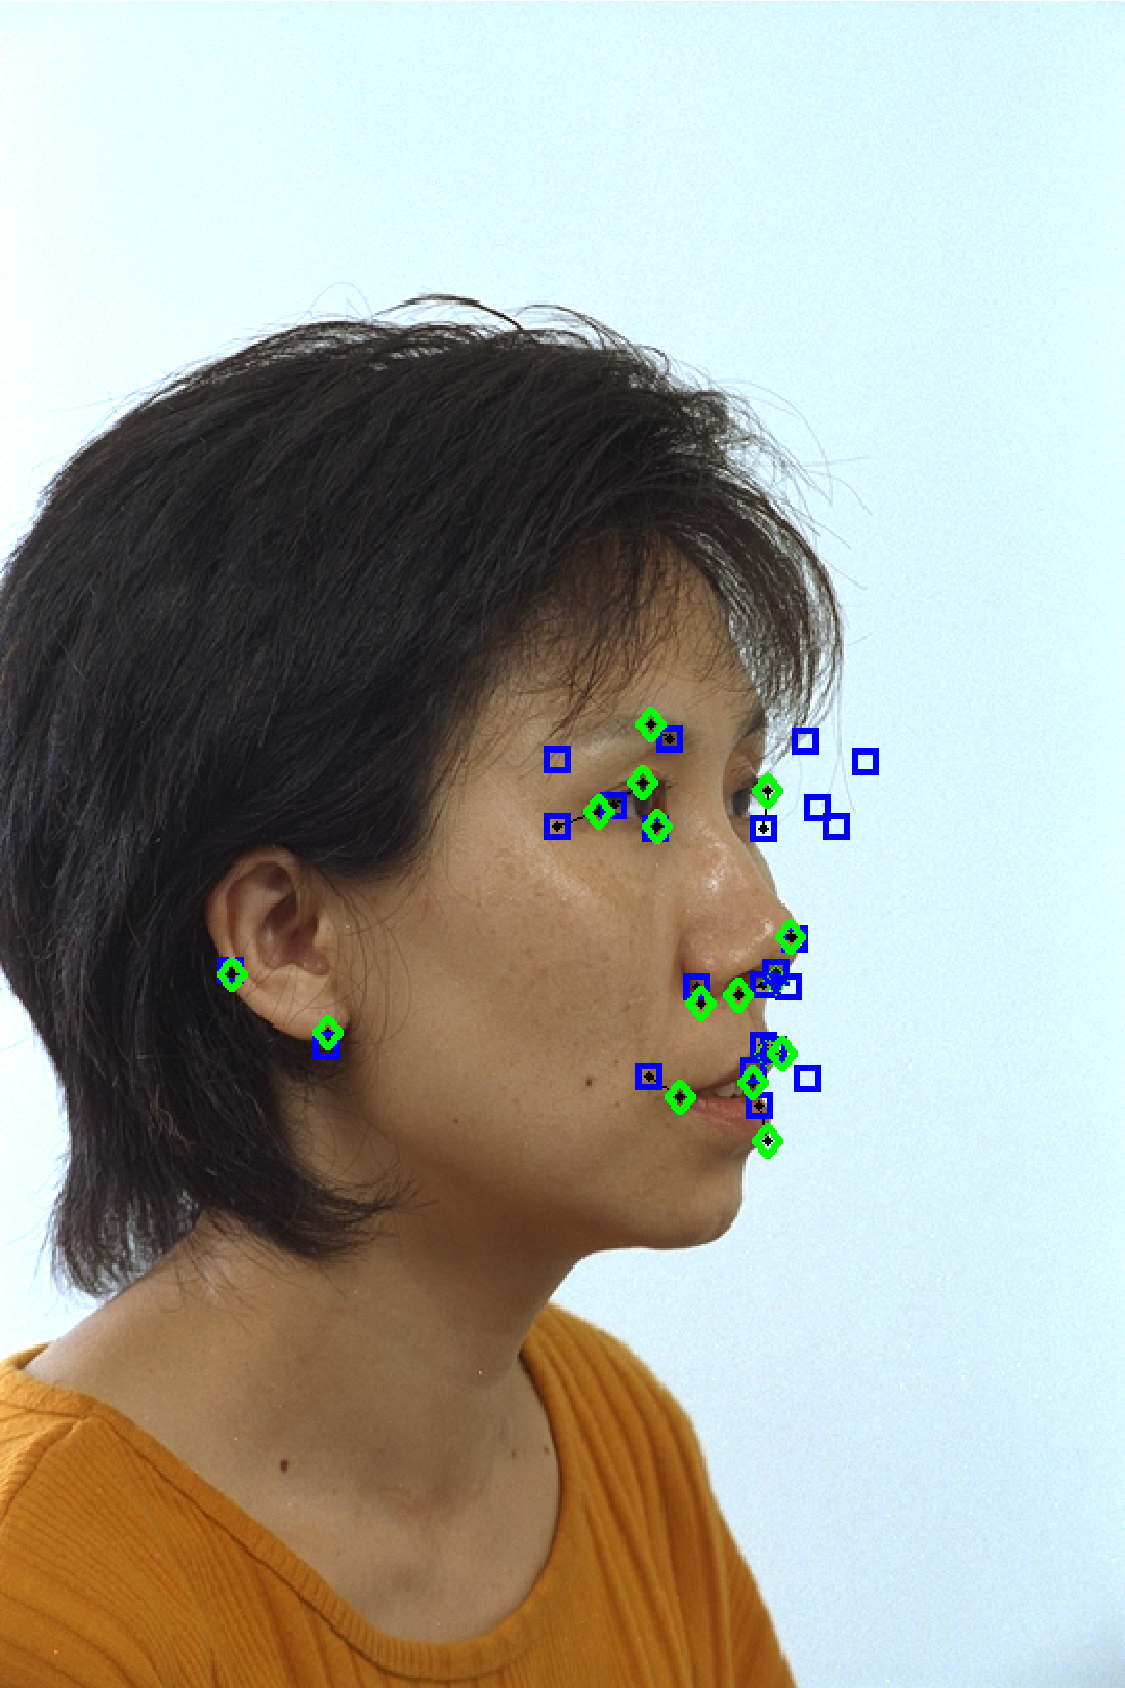
\includegraphics[width=\linewidth]{images/l_hr_success_1.pdf}} &
\parbox[c]{0.11\linewidth}{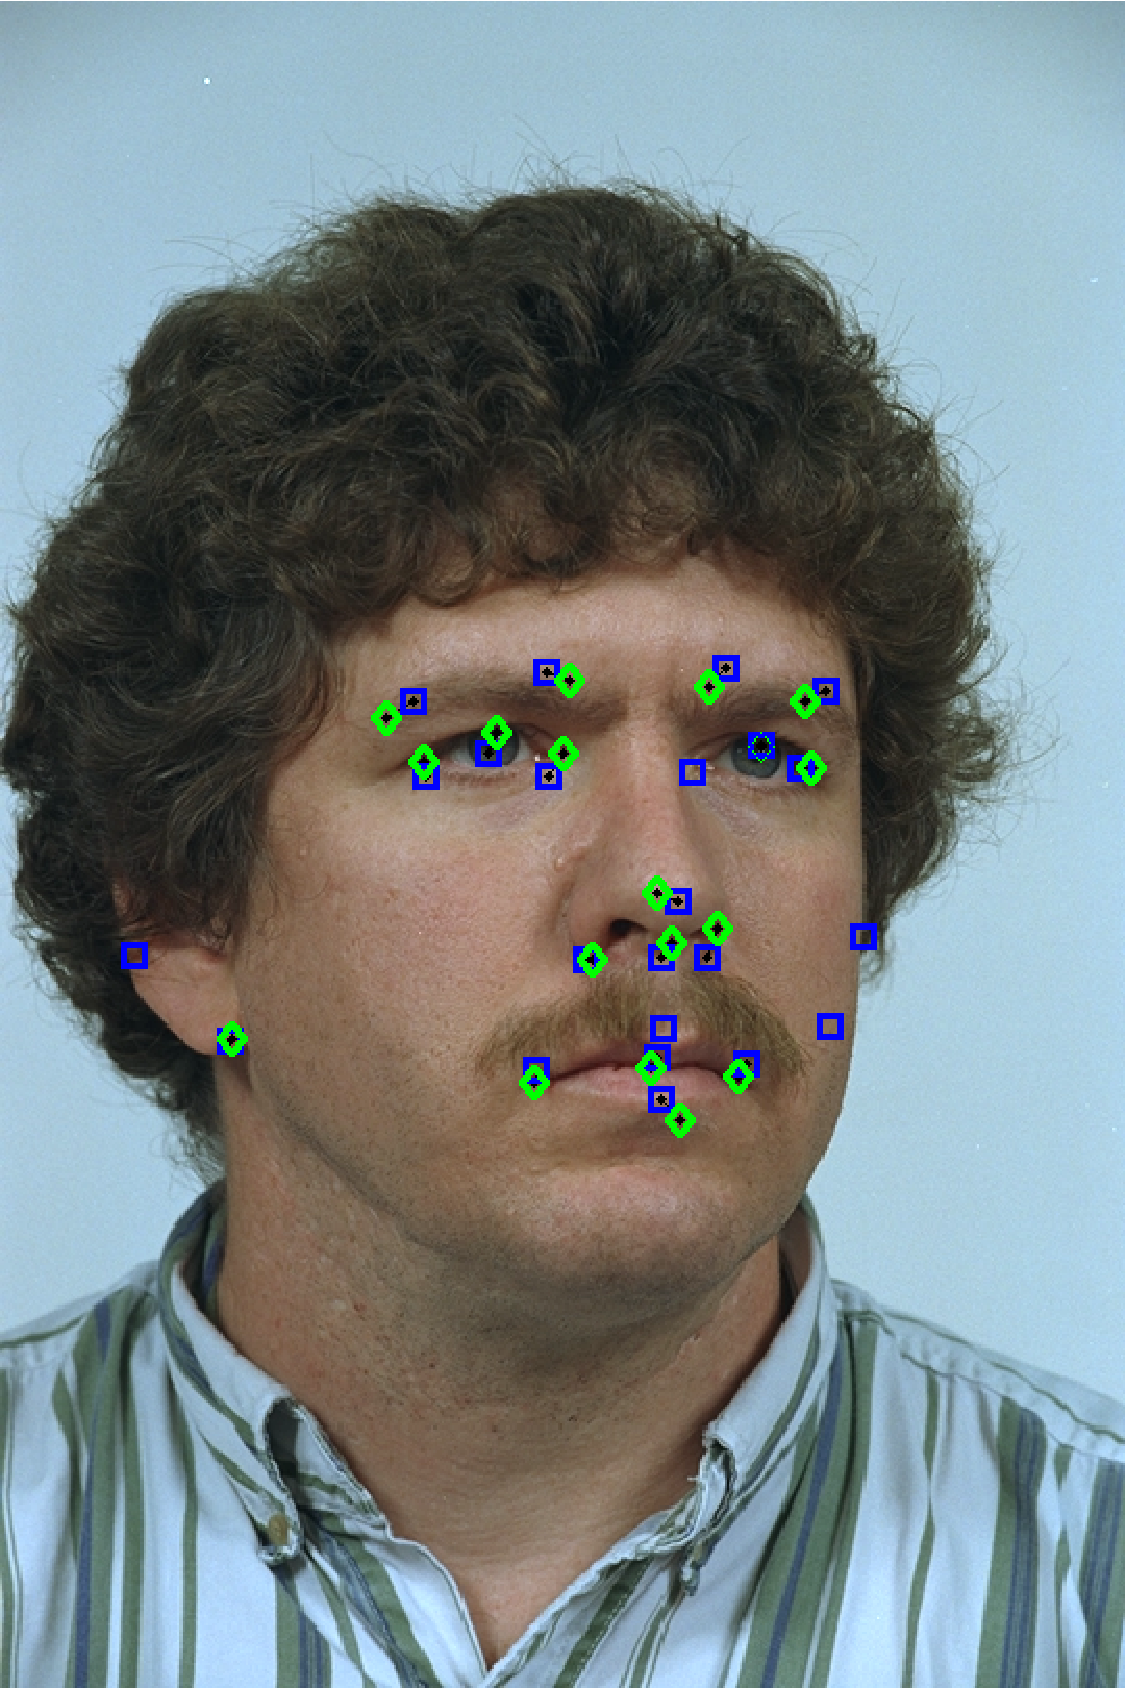
\includegraphics[width=\linewidth]{images/l_rc_success_1.pdf}} \\
&
\parbox[c]{0.11\linewidth}{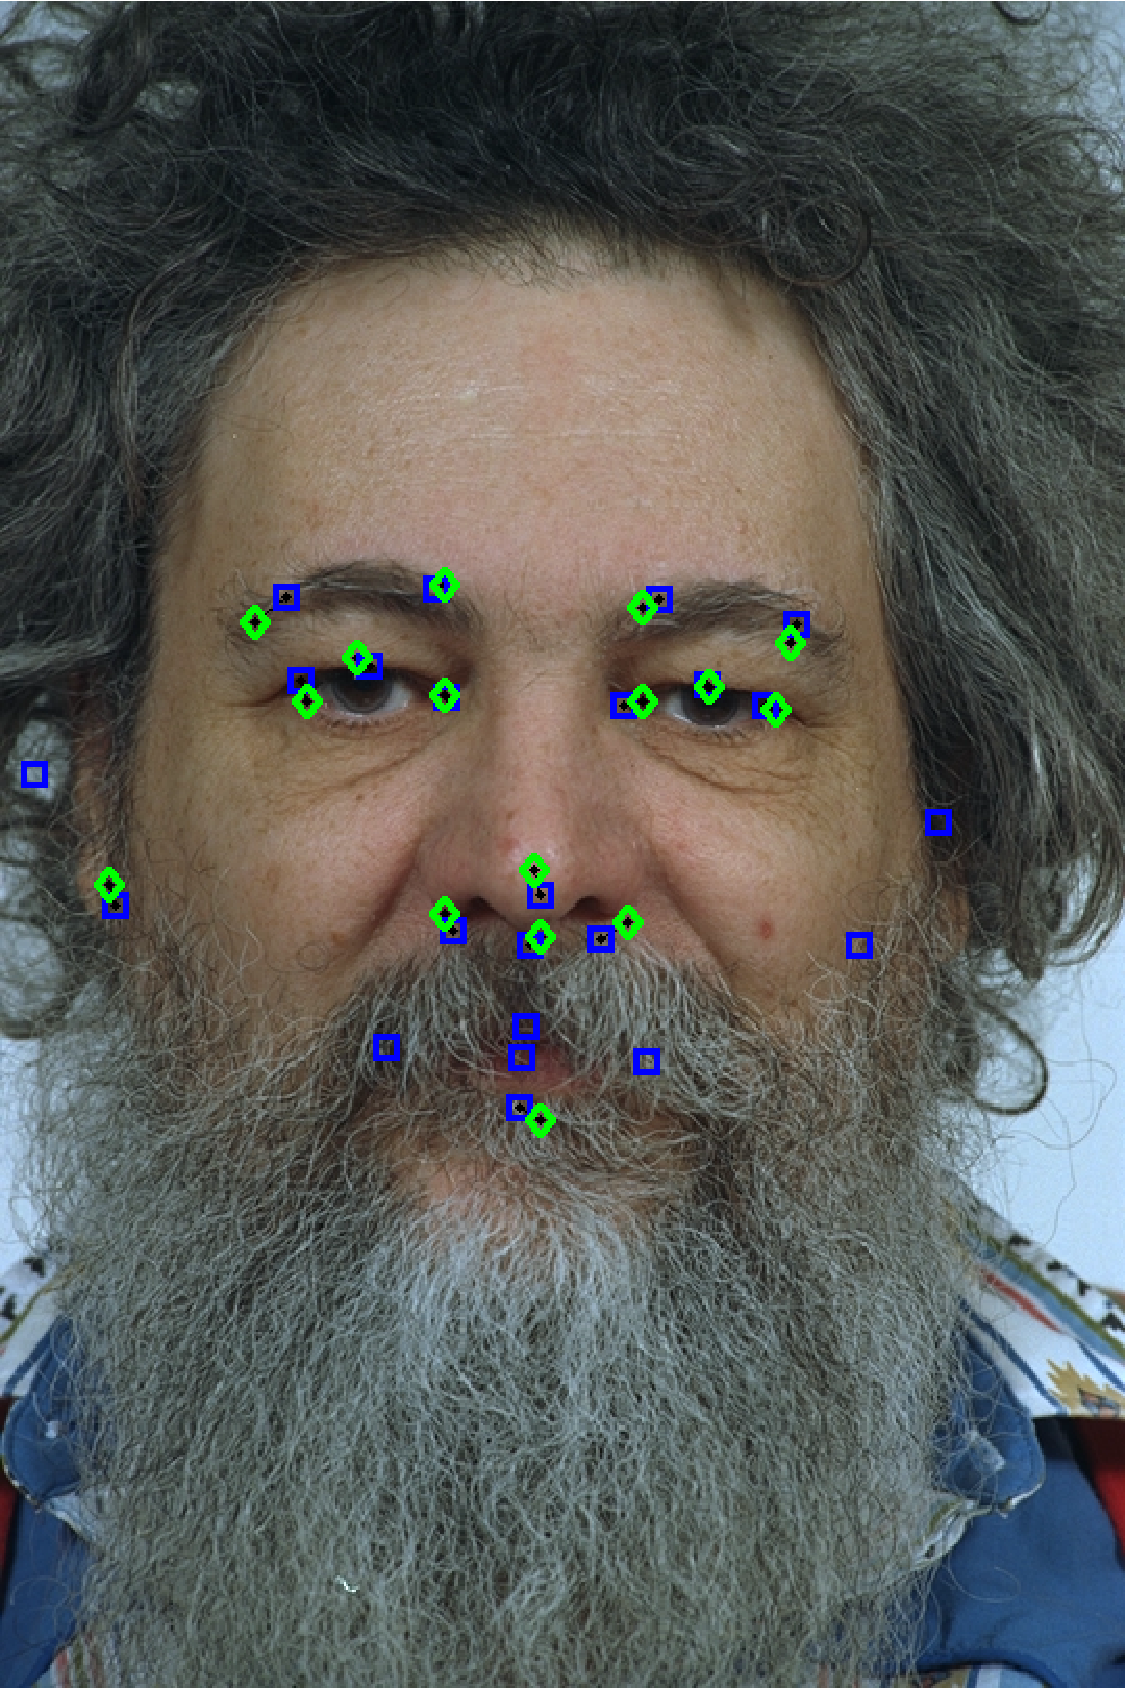
\includegraphics[width=\linewidth]{images/l_fa_success_2.pdf}} &
\parbox[c]{0.11\linewidth}{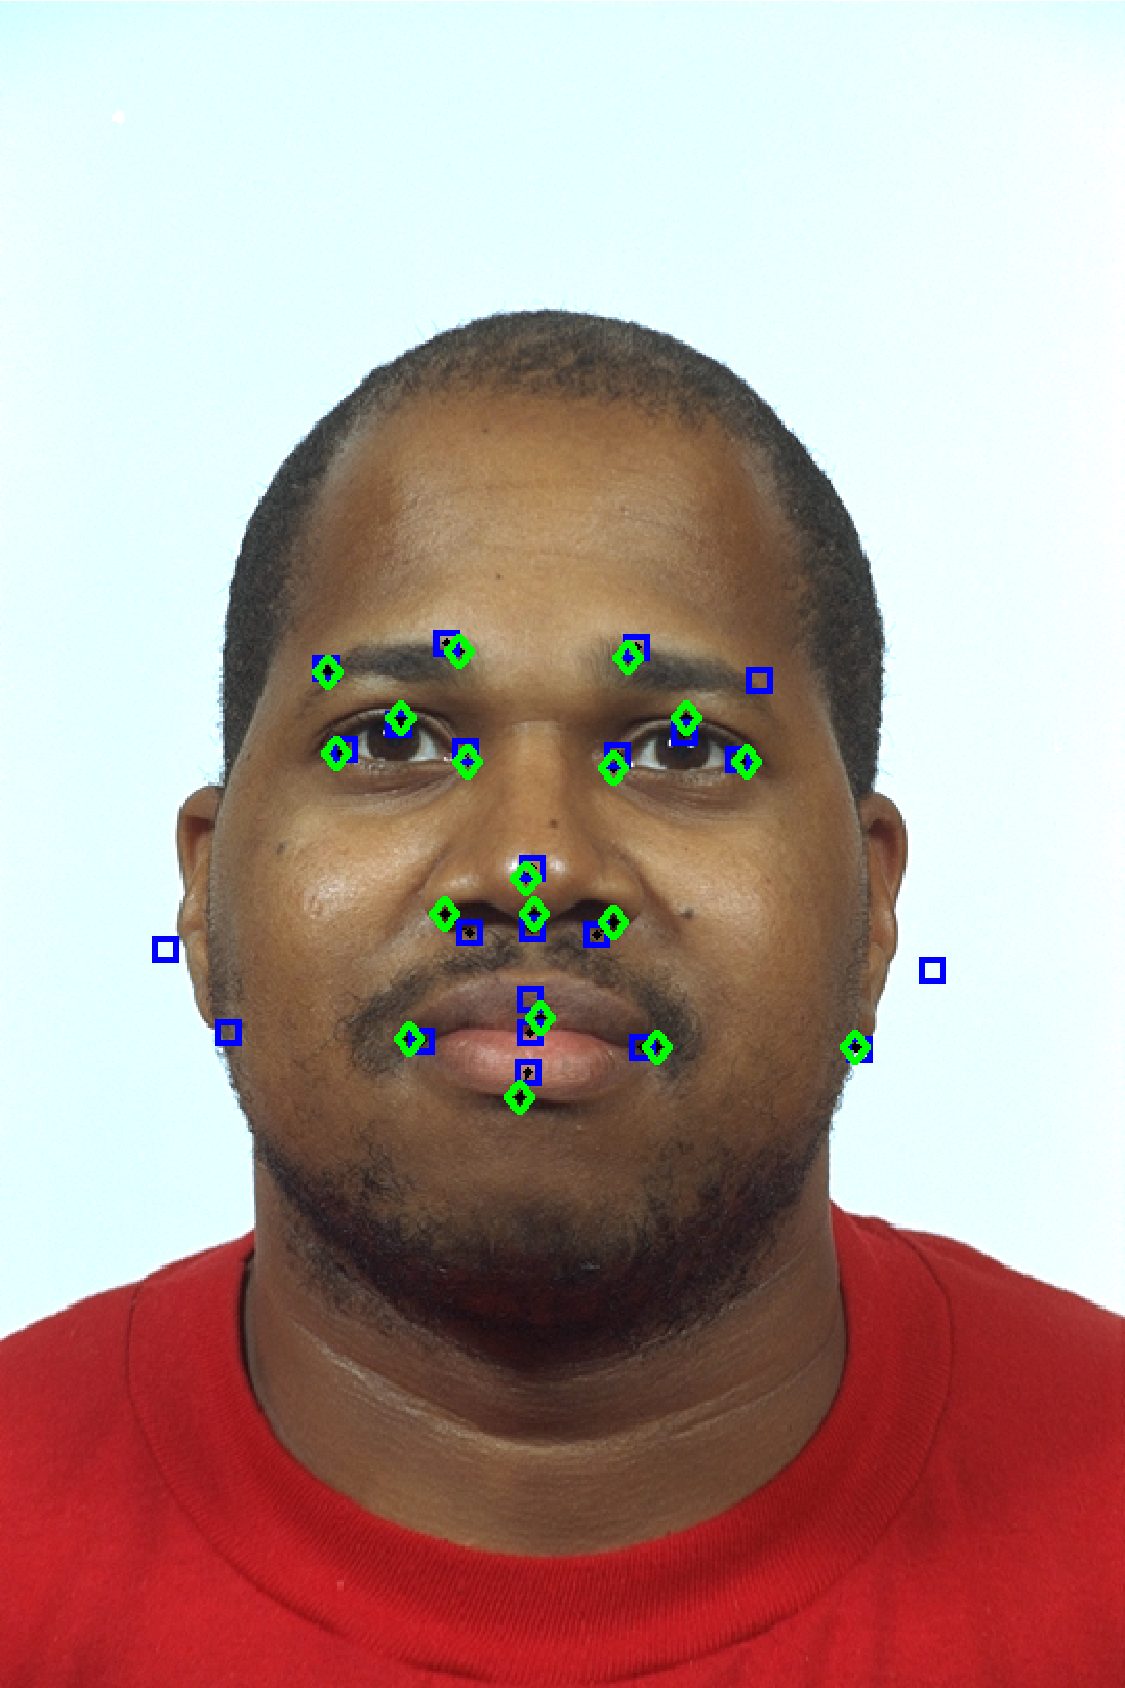
\includegraphics[width=\linewidth]{images/l_fb_success_2.pdf}} &
\parbox[c]{0.11\linewidth}{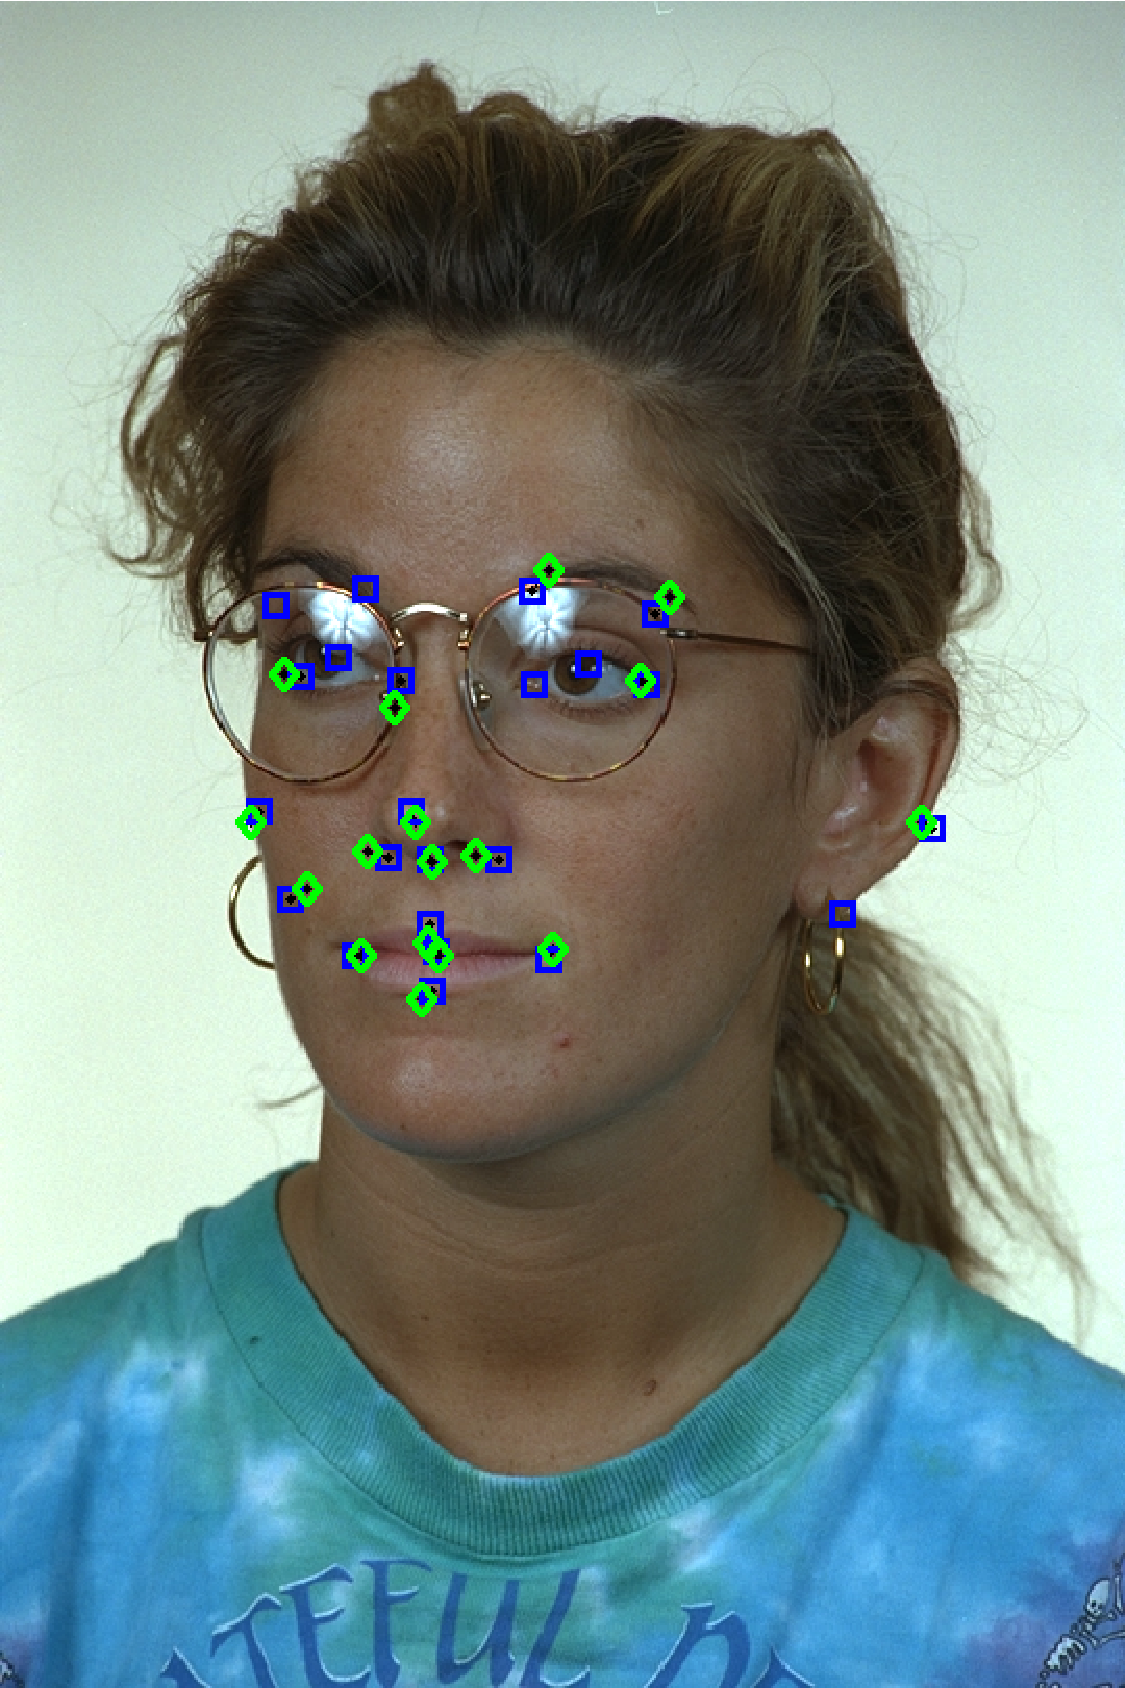
\includegraphics[width=\linewidth]{images/l_ql_success_2.pdf}} &
\parbox[c]{0.11\linewidth}{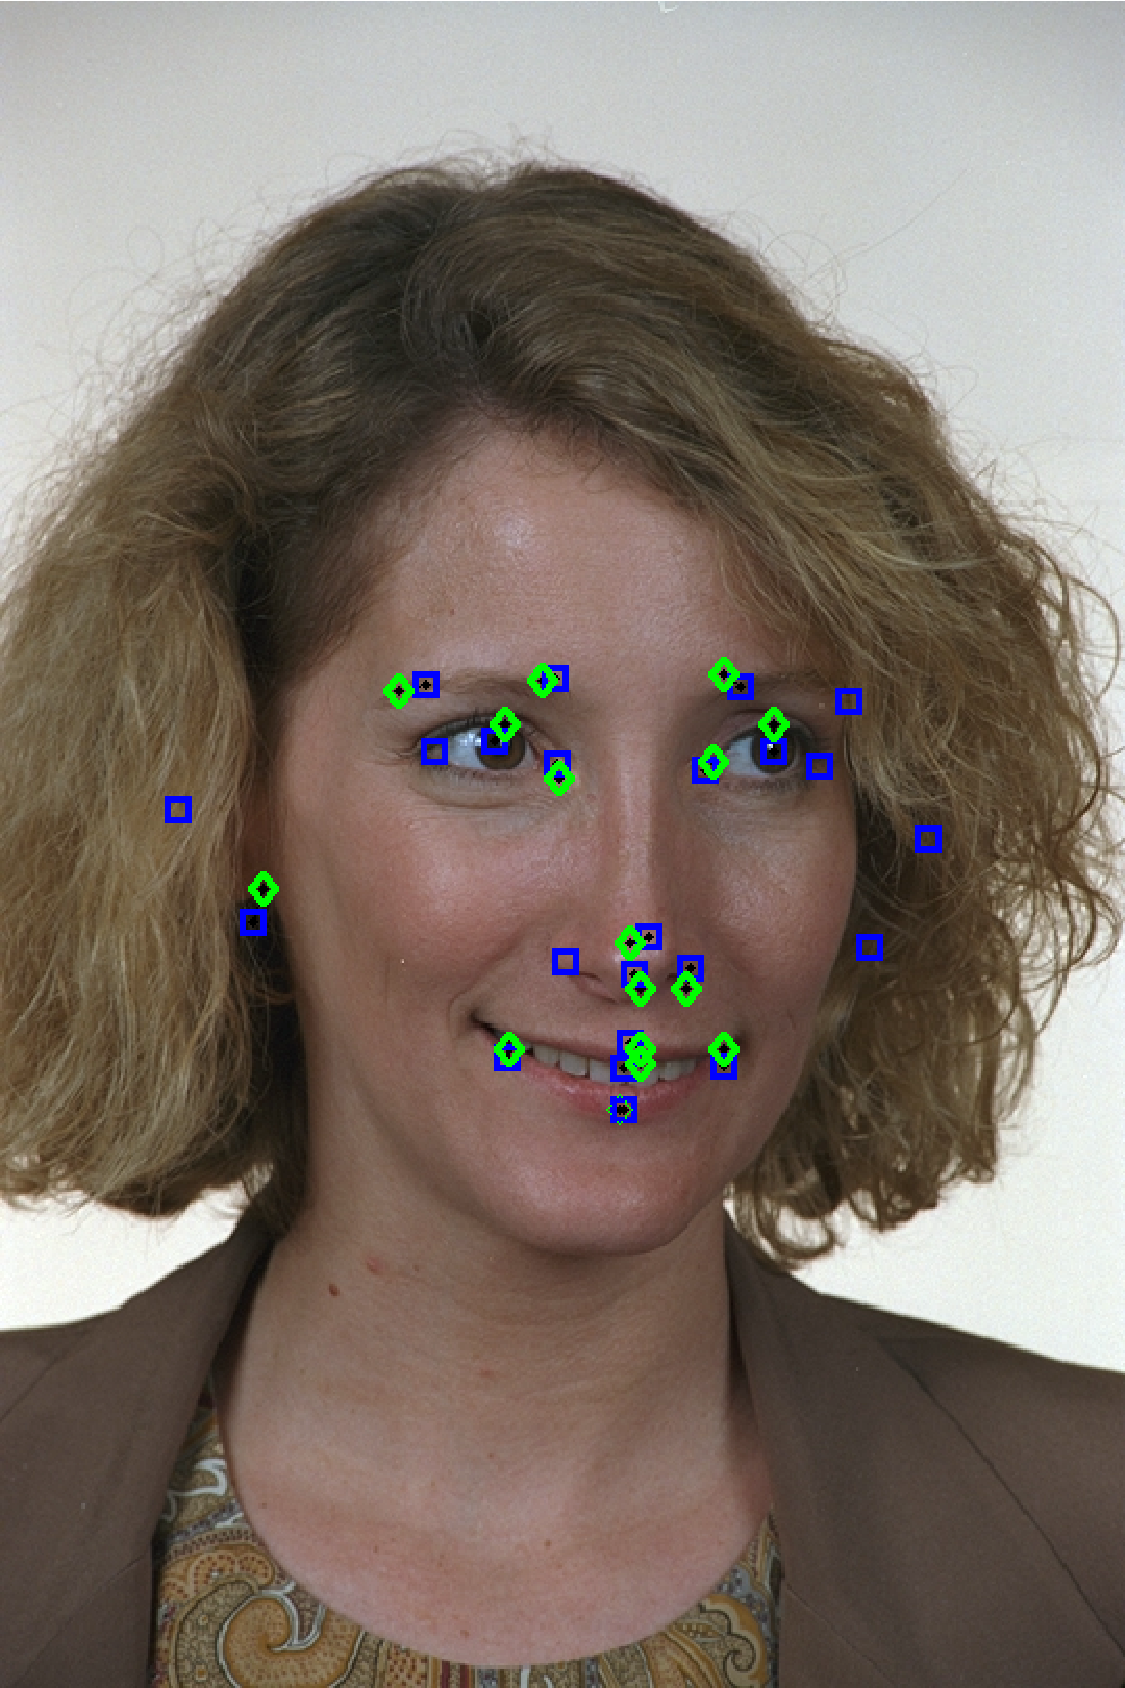
\includegraphics[width=\linewidth]{images/l_qr_success_2.pdf}} &
\parbox[c]{0.11\linewidth}{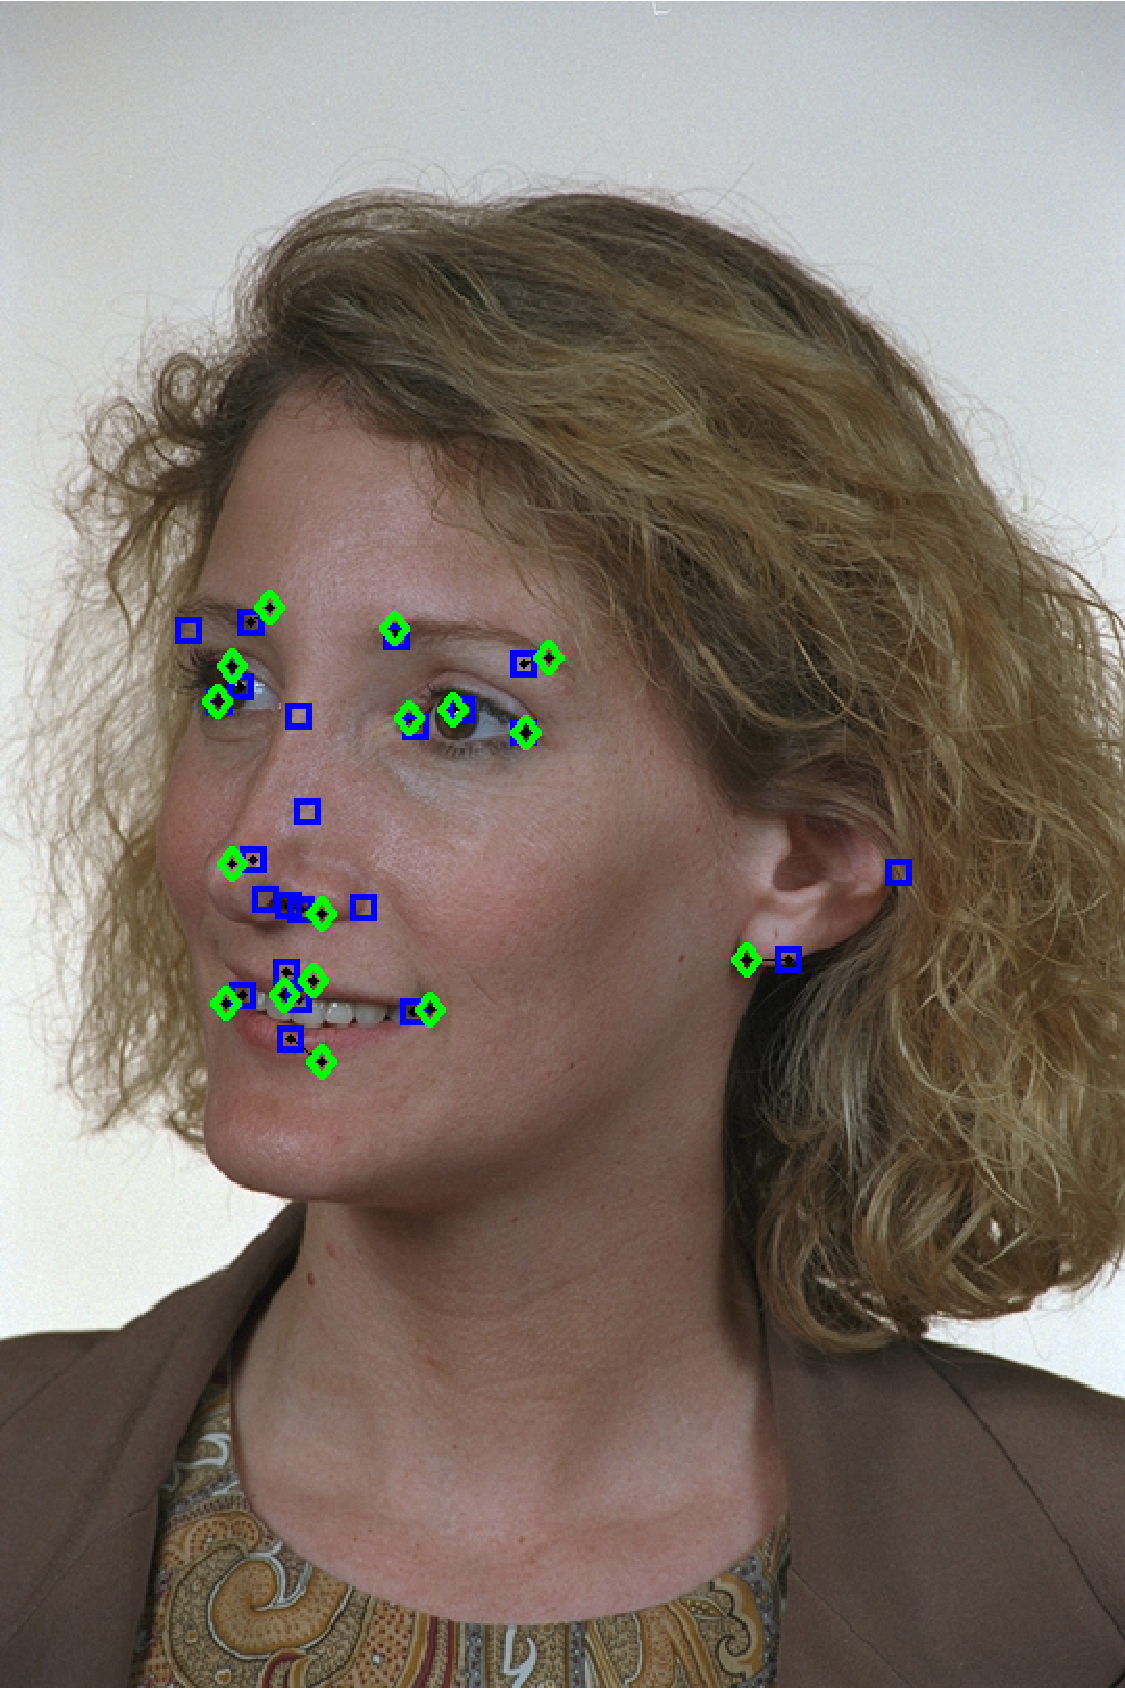
\includegraphics[width=\linewidth]{images/l_hl_success_2.pdf}} &
\parbox[c]{0.11\linewidth}{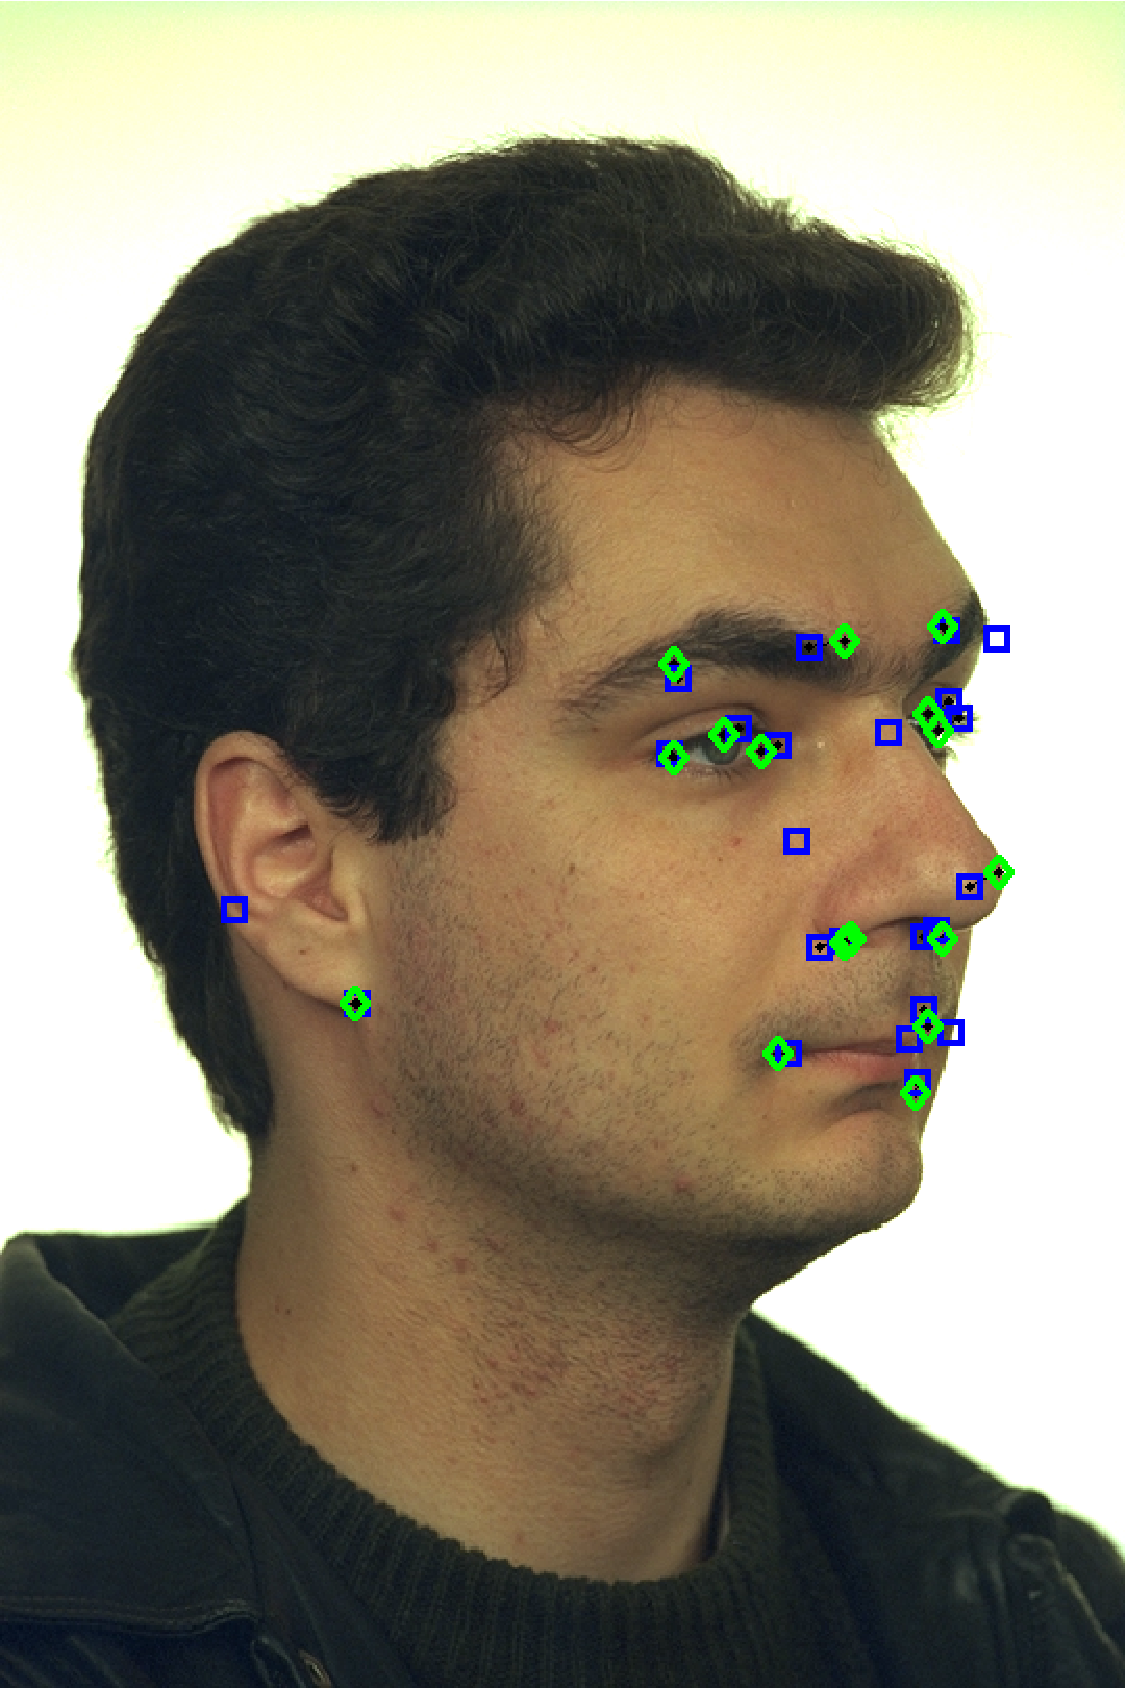
\includegraphics[width=\linewidth]{images/l_hr_success_2.pdf}} &
\parbox[c]{0.11\linewidth}{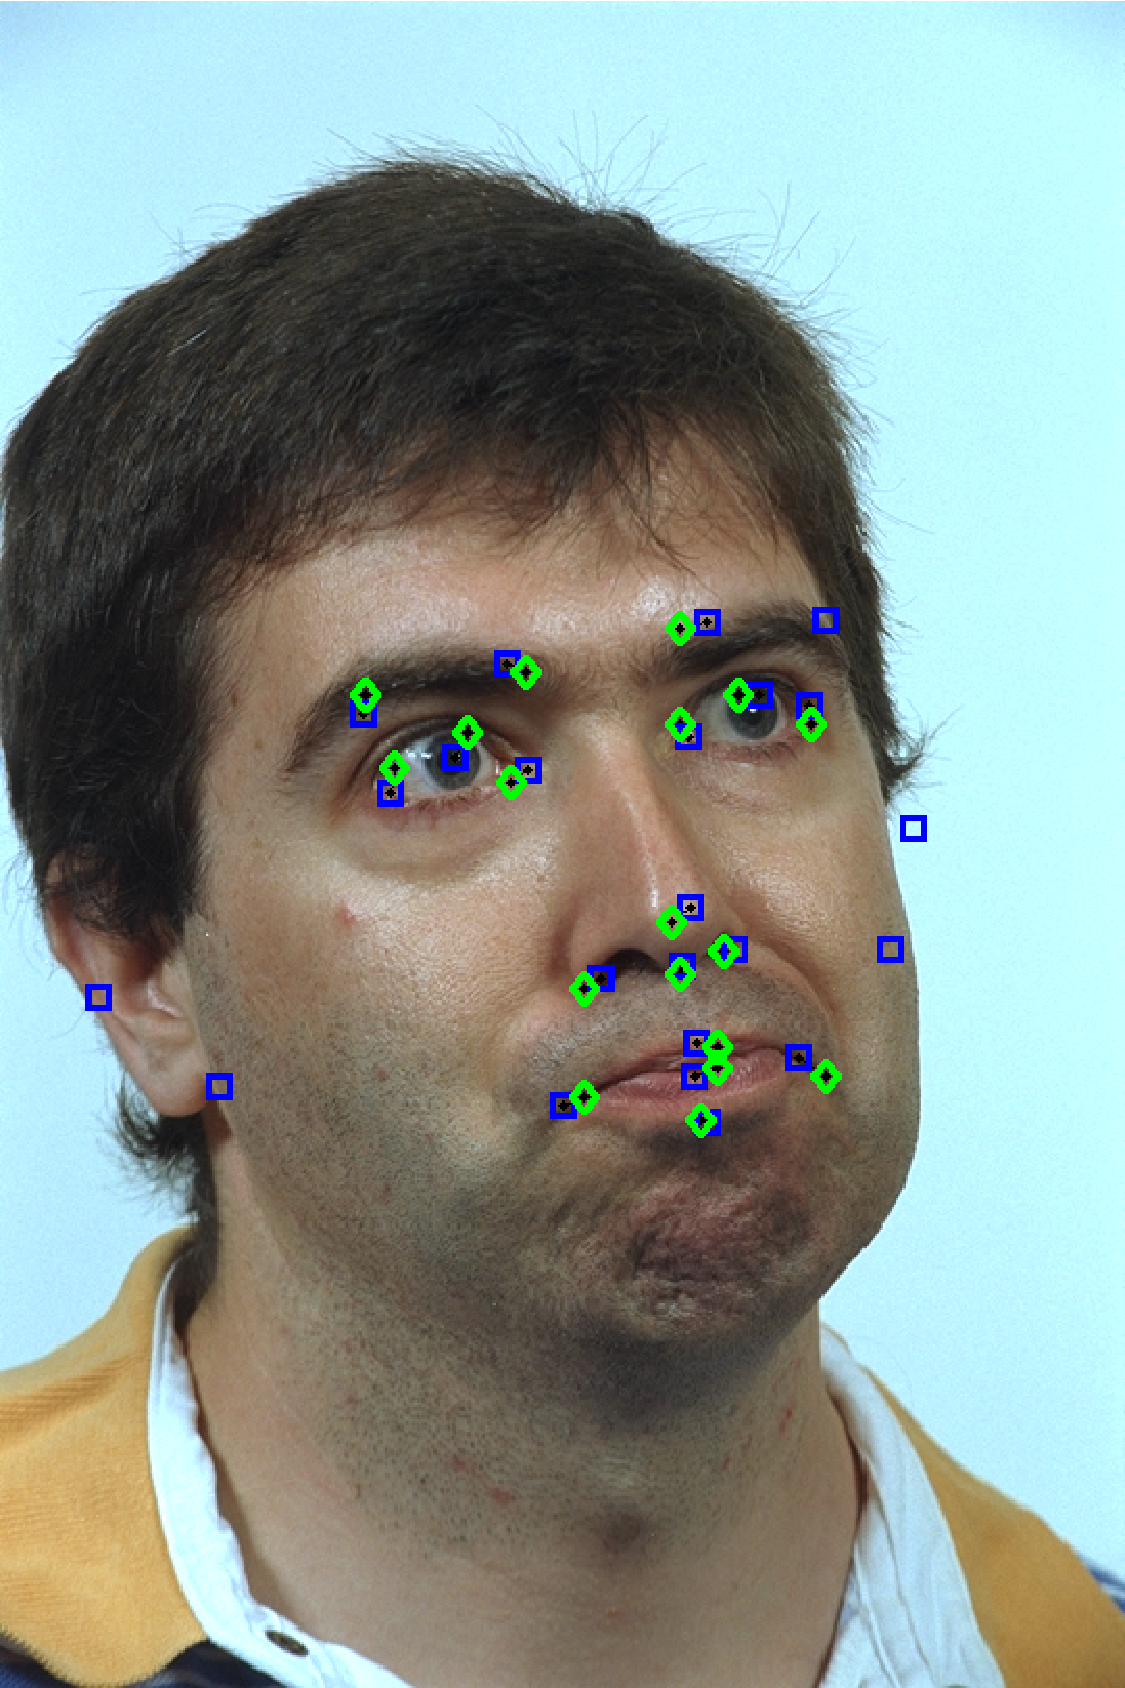
\includegraphics[width=\linewidth]{images/l_rc_success_2.pdf}} \\
\midrule
\begin{sideways}\makebox[0pt][c]{Failure}\end{sideways} &
\parbox[c]{0.11\linewidth}{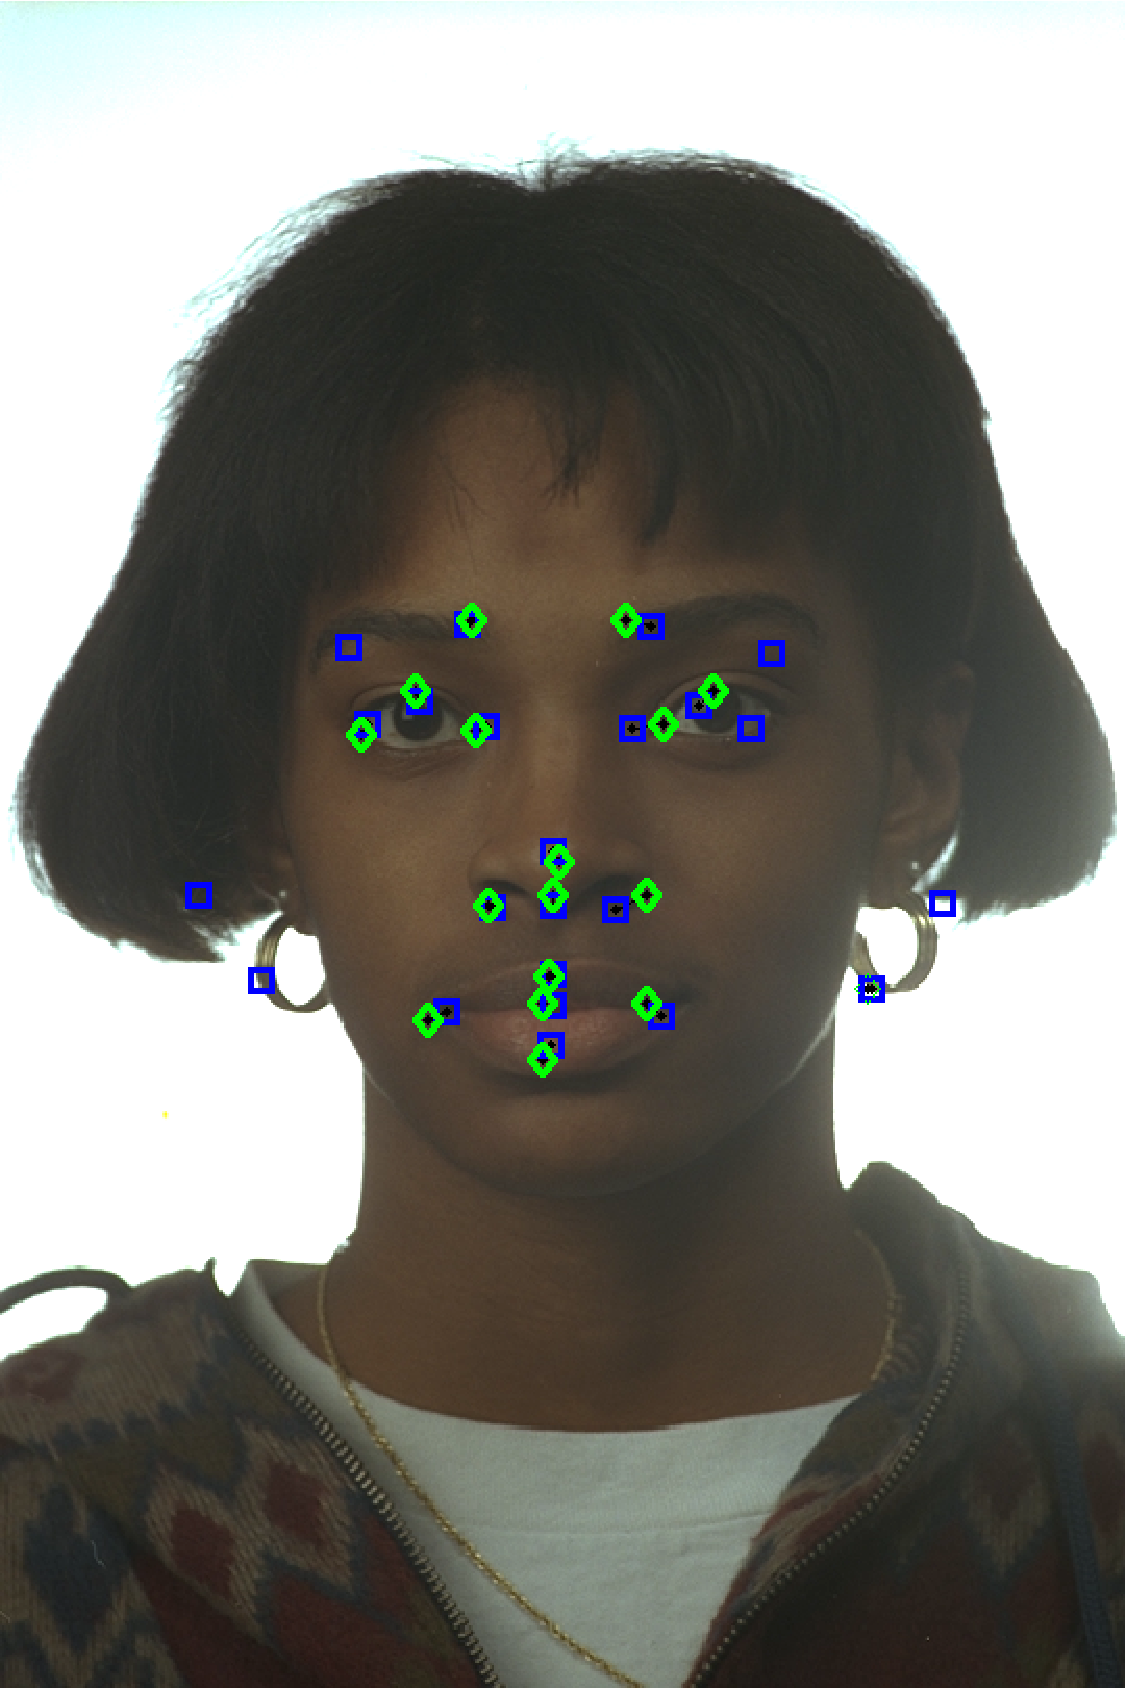
\includegraphics[width=\linewidth]{images/l_fa_fail.pdf}} &
\parbox[c]{0.11\linewidth}{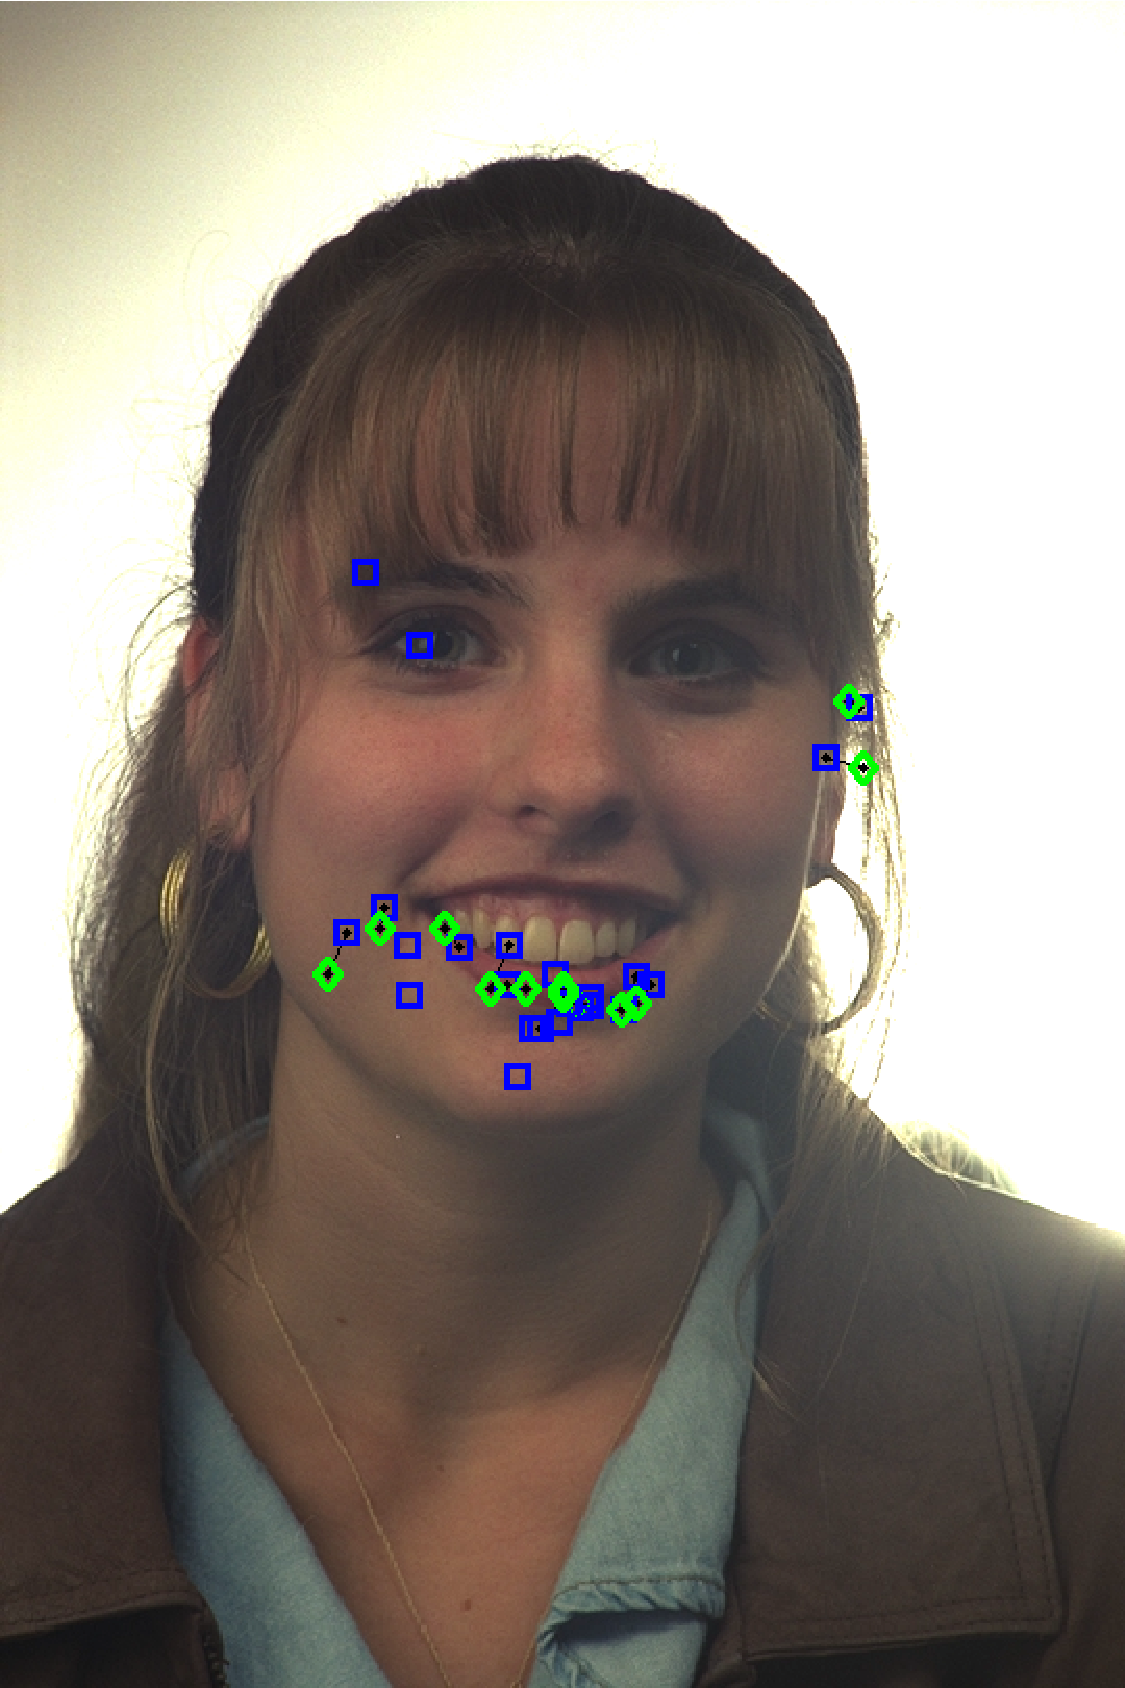
\includegraphics[width=\linewidth]{images/l_fb_fail.pdf}} &
\parbox[c]{0.11\linewidth}{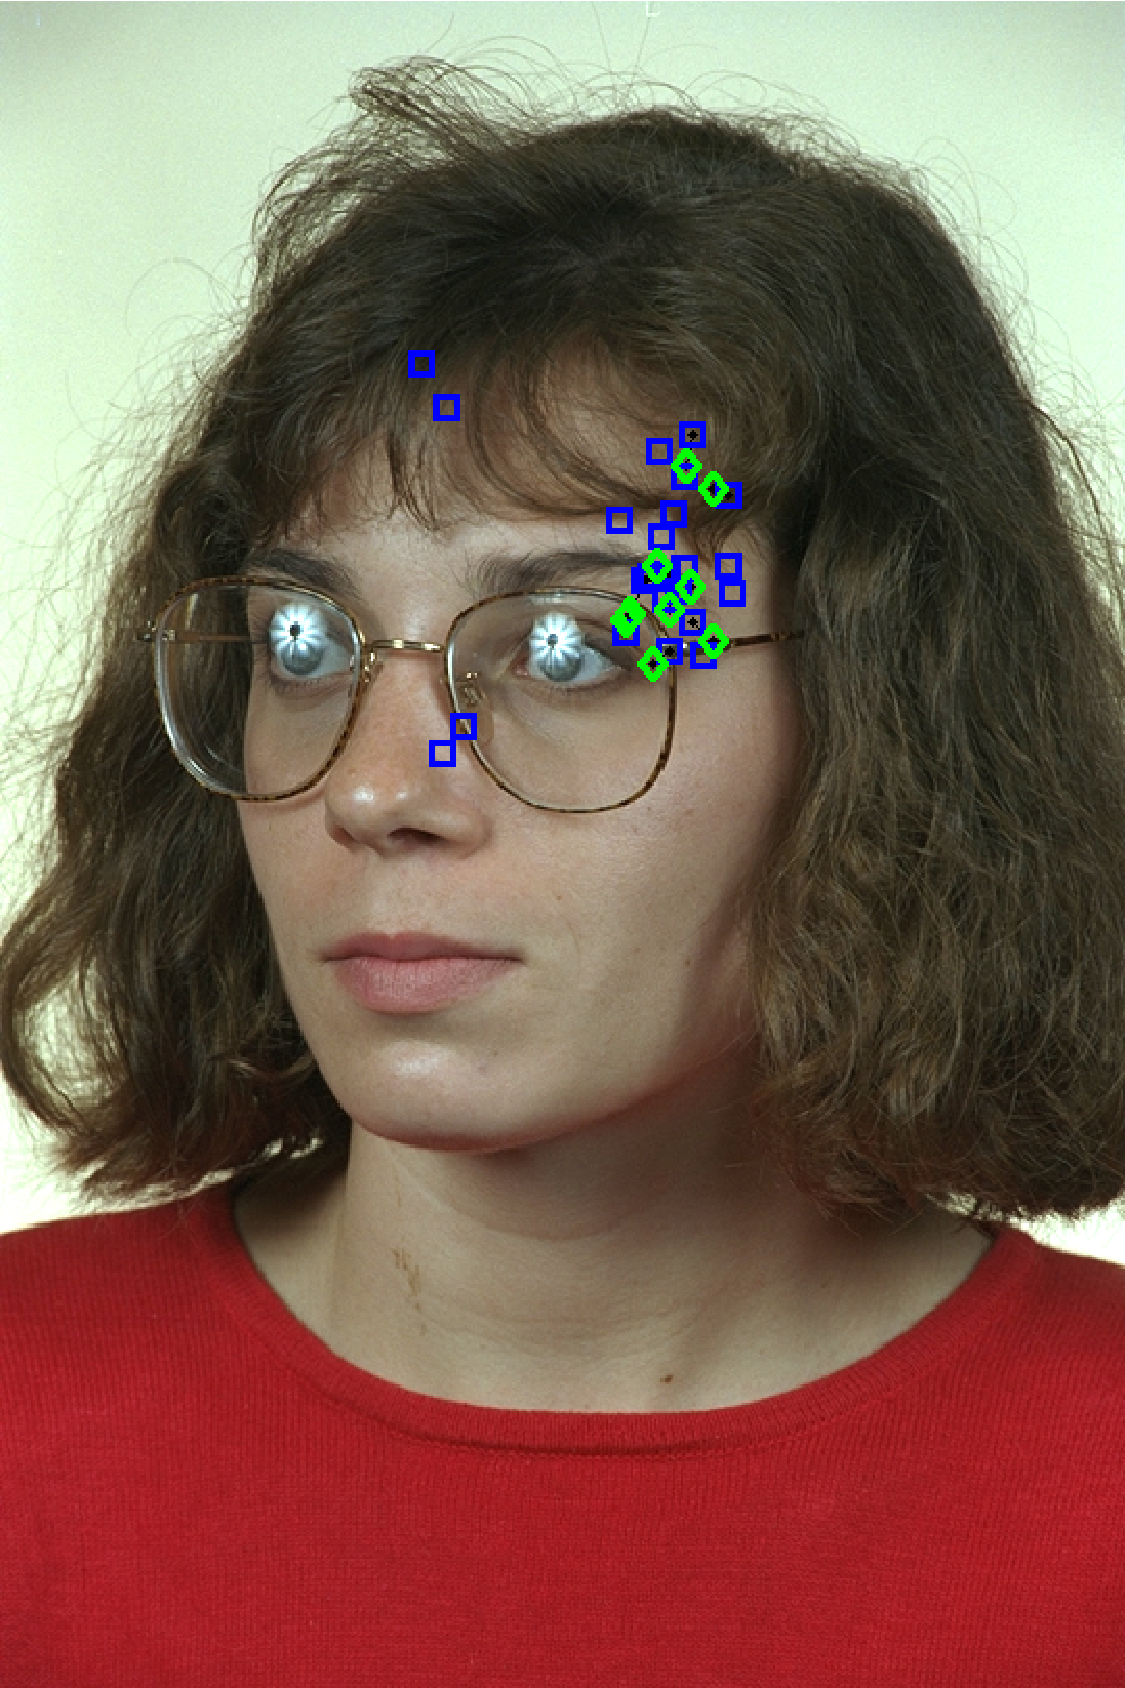
\includegraphics[width=\linewidth]{images/l_ql_fail.pdf}} &
\parbox[c]{0.11\linewidth}{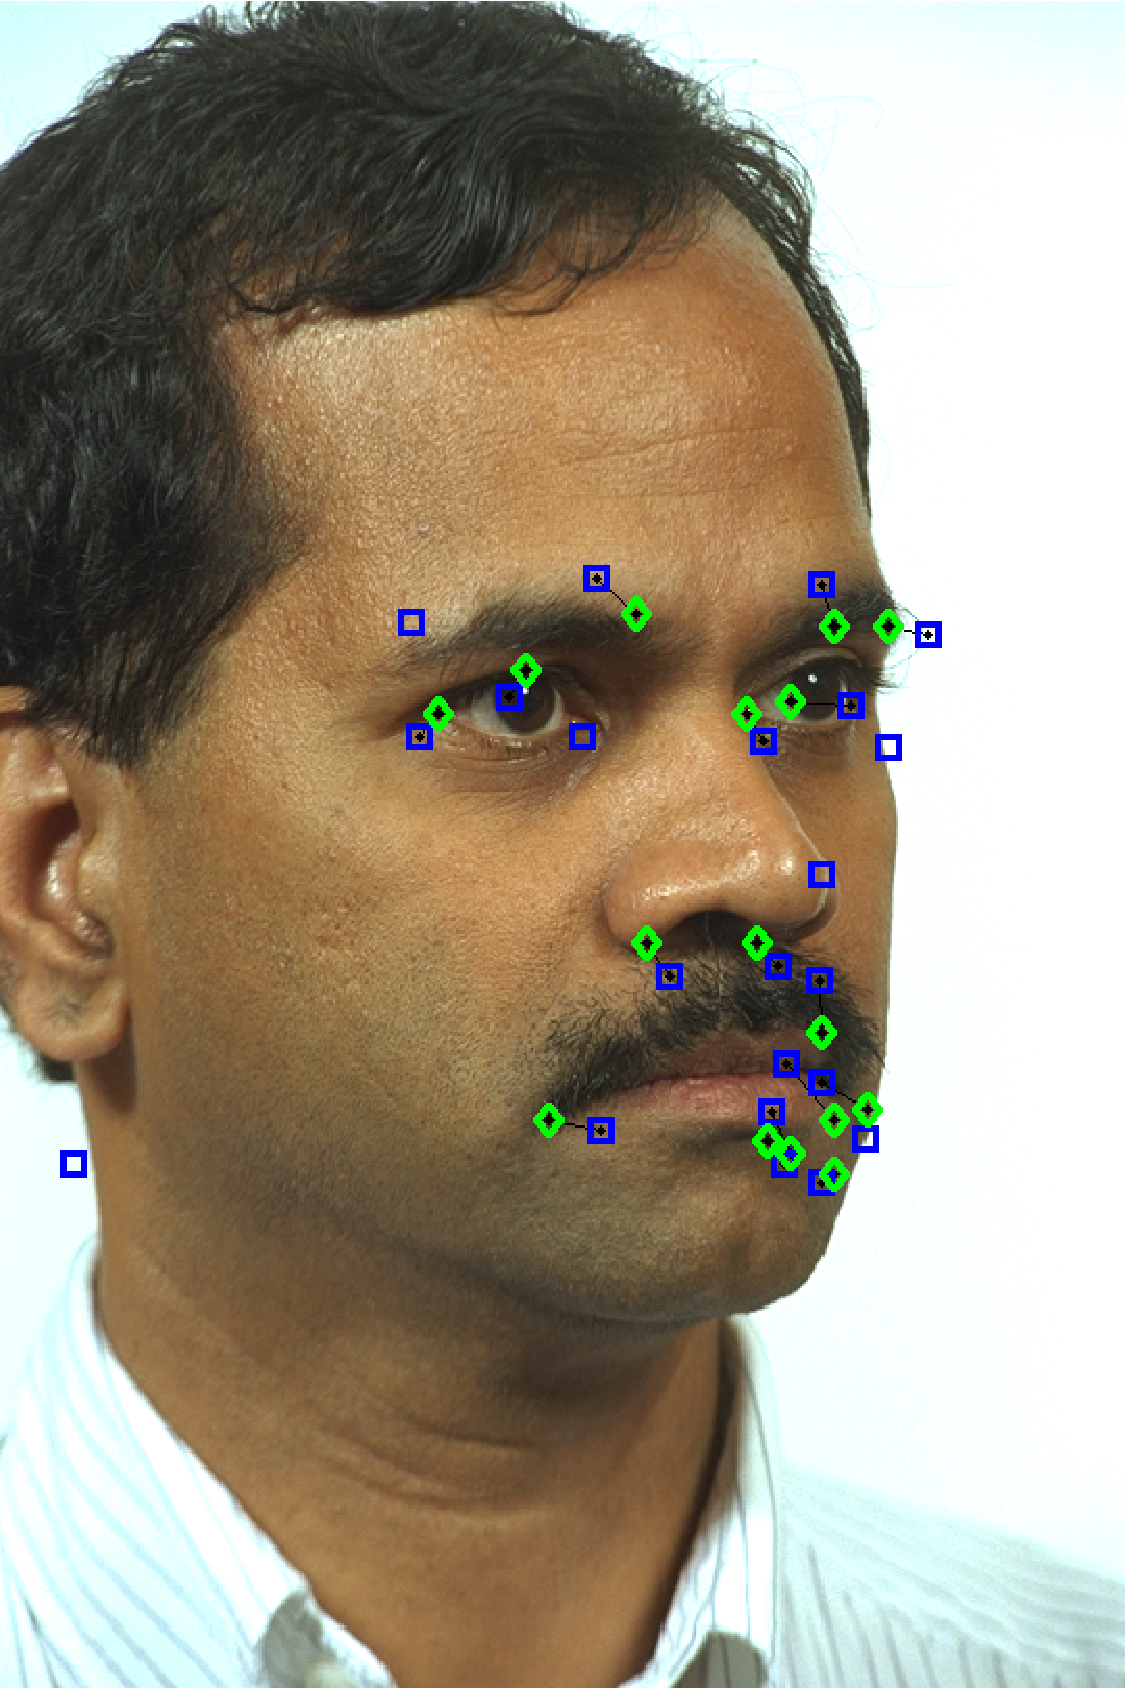
\includegraphics[width=\linewidth]{images/l_qr_fail.pdf}} &
\parbox[c]{0.11\linewidth}{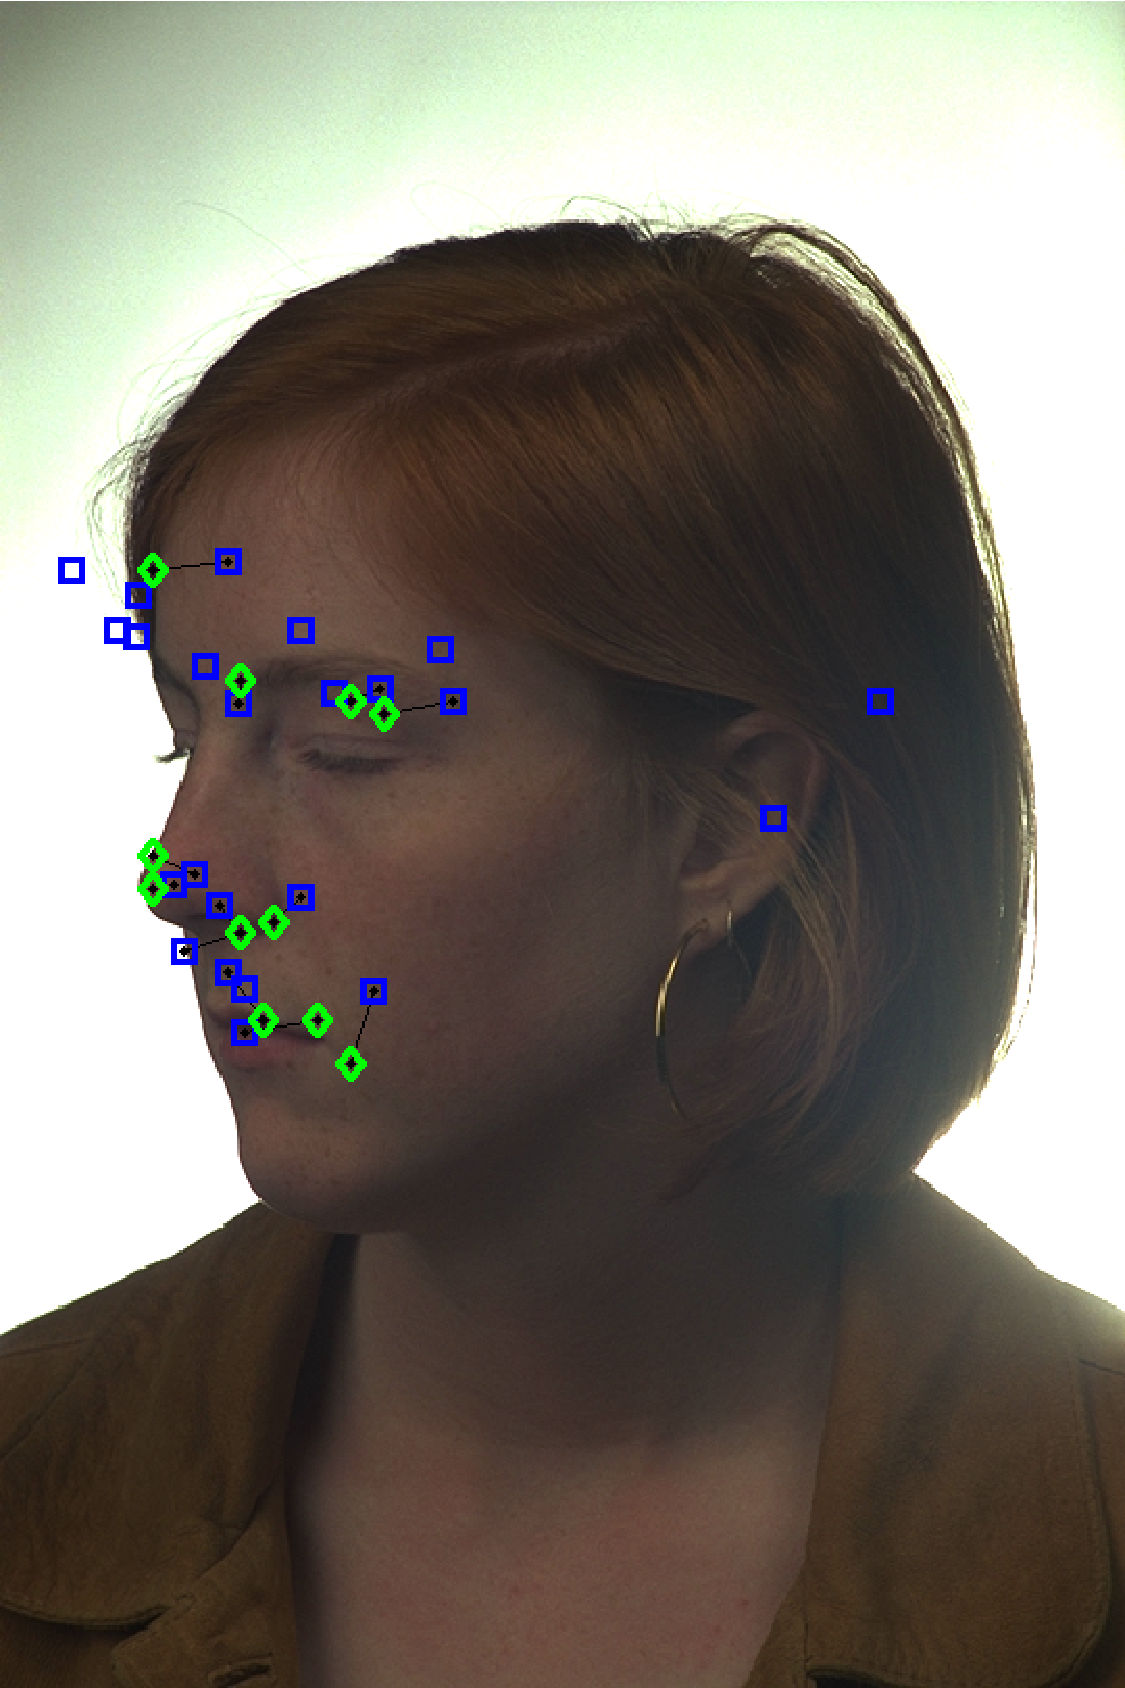
\includegraphics[width=\linewidth]{images/l_hl_fail.pdf}} &
\parbox[c]{0.11\linewidth}{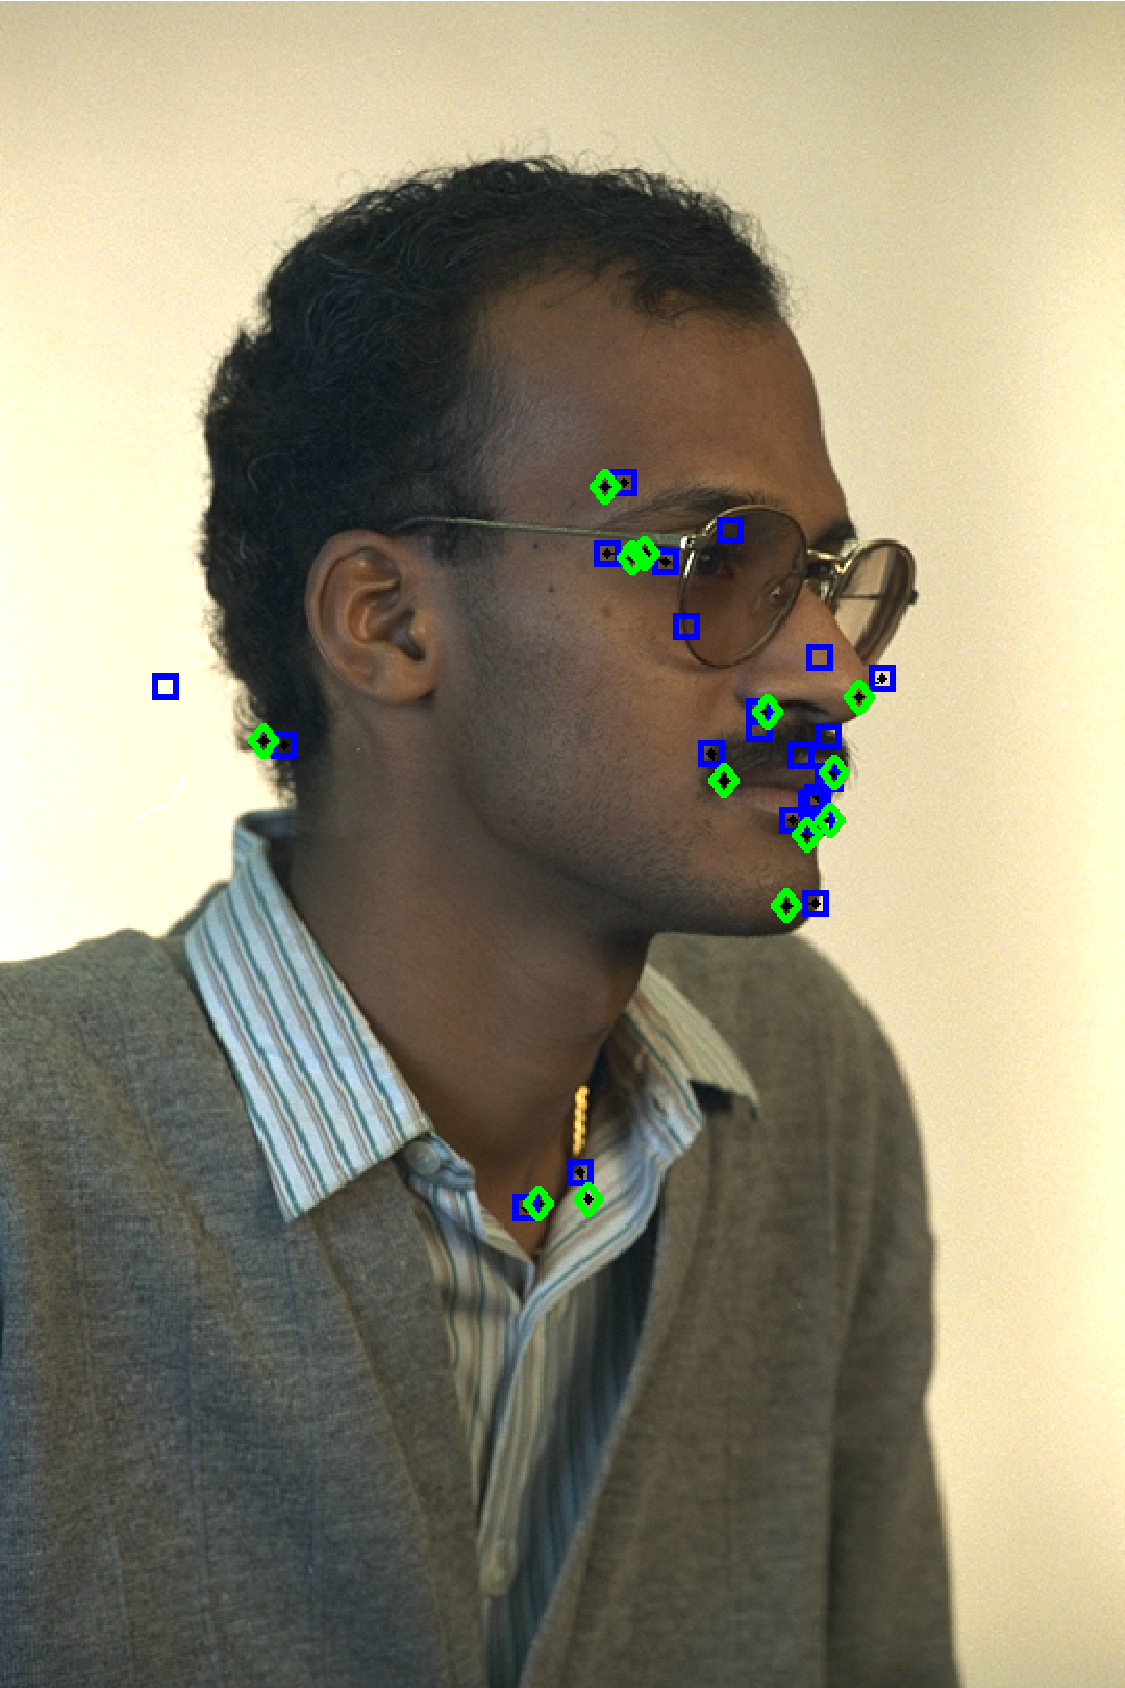
\includegraphics[width=\linewidth]{images/l_hr_fail.pdf}} &
\parbox[c]{0.11\linewidth}{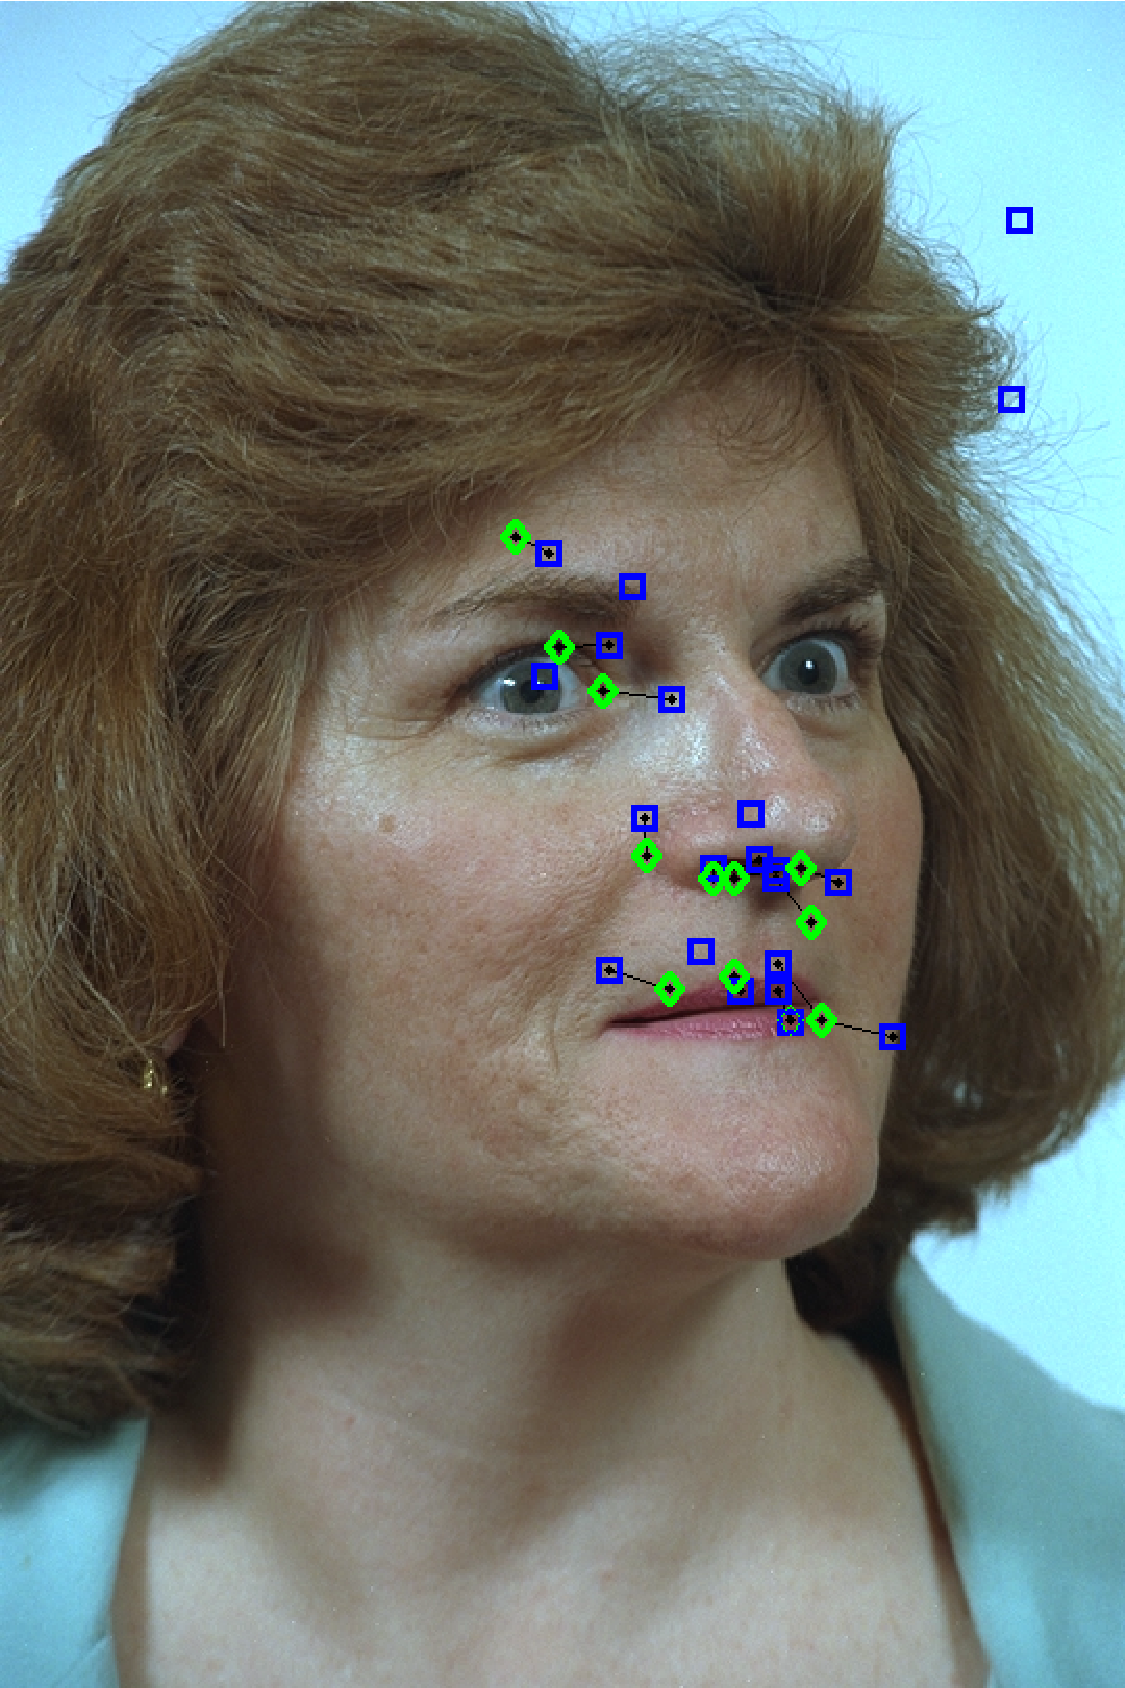
\includegraphics[width=\linewidth]{images/l_rc_fail.pdf}} 
\end{tabular}
  }\\[-1em]
      \begin{multicols}{2}
Some randomly chosen images from the color feret database for each
pose, and the detected landmark positions. The first two rows are success
cases, the last row shows a failure case. 
      \end{multicols}
}
%%%%%%%%%%%%%%%%%%%%%%%%%%%%%%%%%%%%%%%%%%%%%%%%%%%%%%%%%%%%%%%%%%%%%%%%%%%%%%
  \headerbox{Representation}{name=representation,column=2,below=results}{
%%%%%%%%%%%%%%%%%%%%%%%%%%%%%%%%%%%%%%%%%%%%%%%%%%%%%%%%%%%%%%%%%%%%%%%%%%%%%%
\centering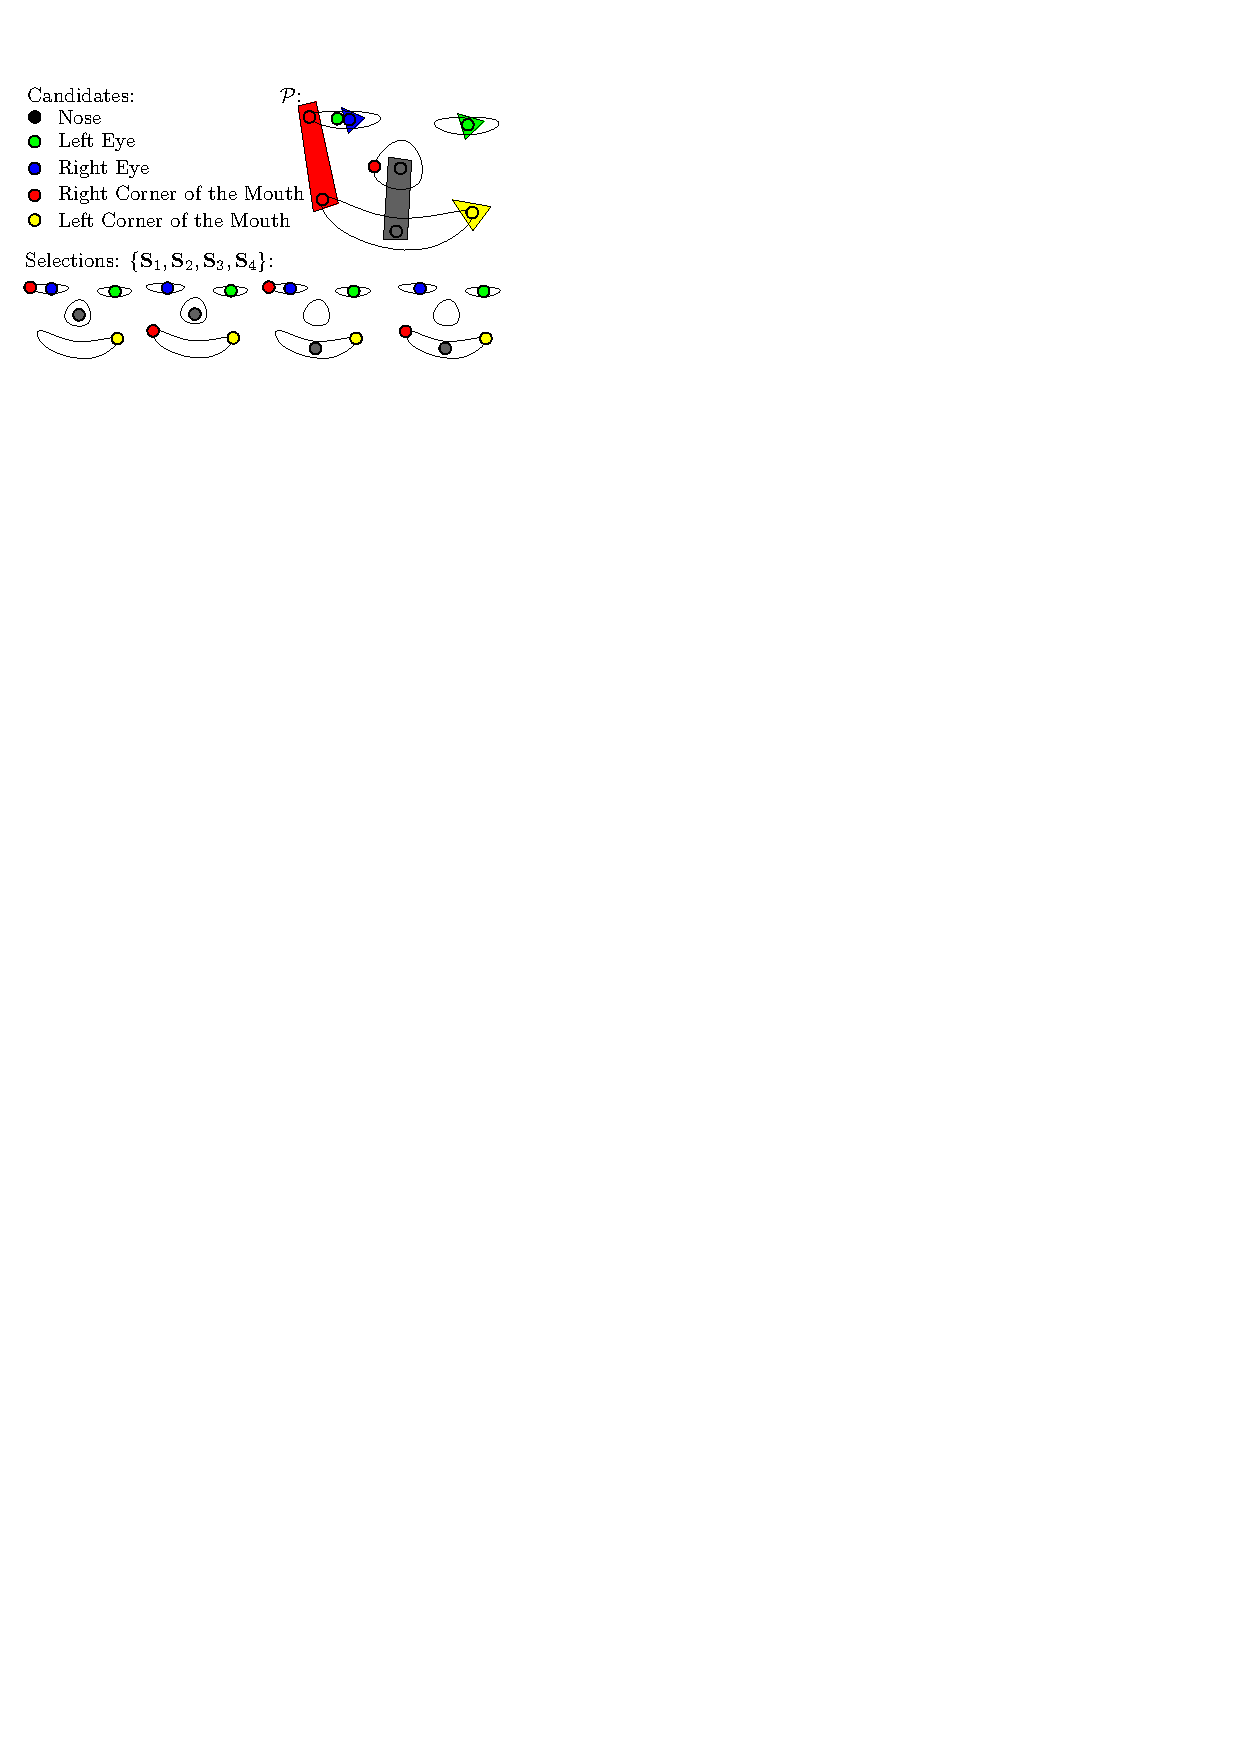
\includegraphics[width=\linewidth]{images/representation.pdf}
Subsets of solutions are encoded as the Kartesian product of subsets of landmark candidates per fiducial point. 
  }
%%%%%%%%%%%%%%%%%%%%%%%%%%%%%%%%%%%%%%%%%%%%%%%%%%%%%%%%%%%%%%%%%%%%%%%%%%%%%%
\headerbox{Scaling Behaviour}{name=scaling,column=2,below=representation}{%
%%%%%%%%%%%%%%%%%%%%%%%%%%%%%%%%%%%%%%%%%%%%%%%%%%%%%%%%%%%%%%%%%%%%%%%%%%%%%%
  \smaller%
  \centering{Runtime as a function of the number of false positives}\\[0em]%
  \centering{{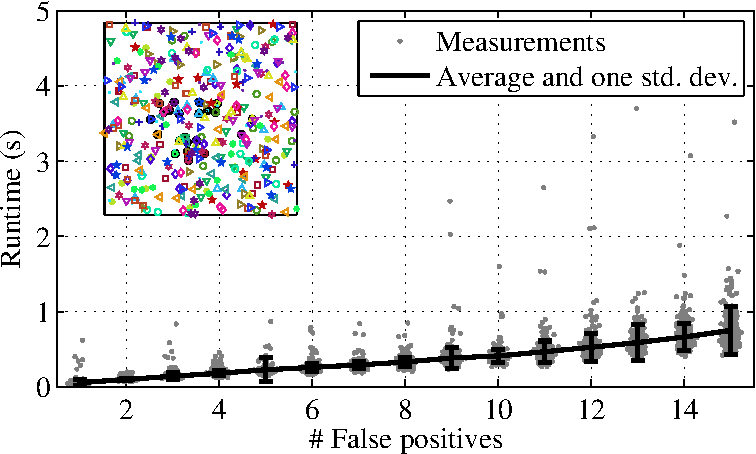
\includegraphics[width=0.9\linewidth]{images/typical_random_no_noise-crop.pdf}}}\\[0em]%
  \centering{Runtime as a function of detection accuracy}\\[0em]%
  \centering{{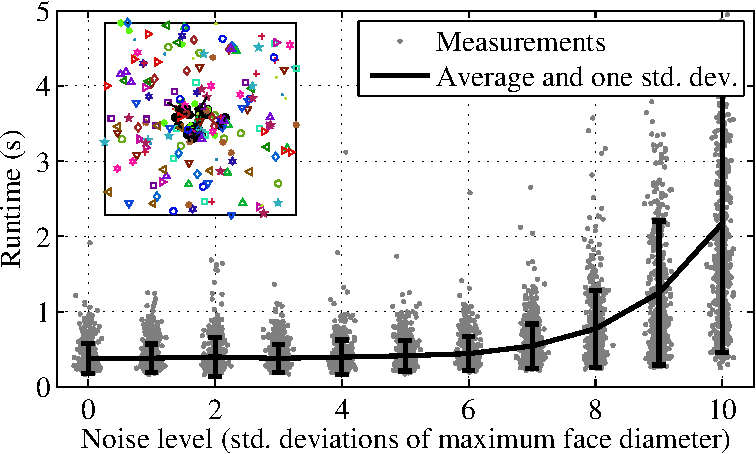
\includegraphics[width=0.9\linewidth]{images/typical_random_add_noise-crop.pdf}}}\\[0em]%
}
%%%%%%%%%%%%%%%%%%%%%%%%%%%%%%%%%%%%%%%%%%%%%%%%%%%%%%%%%%%%%%%%%%%%%%%%%%%%%%
  \headerbox{References}{name=references,column=0,above=bottom}{
%%%%%%%%%%%%%%%%%%%%%%%%%%%%%%%%%%%%%%%%%%%%%%%%%%%%%%%%%%%%%%%%%%%%%%%%%%%%%%
    \smaller
    \bibliographystyle{ieee}
    \renewcommand{\section}[2]{\vskip 0.05em}
      \begin{thebibliography}{1}\itemsep=-0.01em
      \setlength{\baselineskip}{0.4em}
      \bibitem{amberg11:bnb}
        B.~Amberg, T. Vetter.
        \newblock {O}ptimal {L}andmark {D}etection using {S}hape {M}odels and {B}ranch and {B}ound
        \newblock In {\em ICCV '11}
      \end{thebibliography}
   \vspace{0.3em}
  }
%%%%%%%%%%%%%%%%%%%%%%%%%%%%%%%%%%%%%%%%%%%%%%%%%%%%%%%%%%%%%%%%%%%%%%%%%%%%%%
  \headerbox{Source Code}{name=source,column=2,above=bottom}{
%%%%%%%%%%%%%%%%%%%%%%%%%%%%%%%%%%%%%%%%%%%%%%%%%%%%%%%%%%%%%%%%%%%%%%%%%%%%%%
  \noindent
  \begin{minipage}{\linewidth}
  \begin{minipage}{0.75\linewidth}
    \indent{}The source code is available at \\
    \url{http://www.cs.unibas.ch/personen/amberg_brian/bnb/}
  \end{minipage}\hfill%
  \begin{minipage}{0.23\linewidth}
  \hfill
\includegraphics[width=\linewidth]{chart}
  \end{minipage}
  \end{minipage}
  }
%%%%%%%%%%%%%%%%%%%%%%%%%%%%%%%%%%%%%%%%%%%%%%%%%%%%%%%%%%%%%%%%%%%%%%%%%%%%%%
  \headerbox{Formulation}{name=formulation,column=0,below=contribution,above=references}{
%%%%%%%%%%%%%%%%%%%%%%%%%%%%%%%%%%%%%%%%%%%%%%%%%%%%%%%%%%%%%%%%%%%%%%%%%%%%%%
The solution is constrained by a shape model
\begin{align}
  M(\Params) &= (m_1(\Params), \dots, m_N(\Params))\\
   m_i &: \SRR^{N_{\Params}}\to\SRR^2\nonumber
\end{align}
mapping model parameters~$\Params$ to image positions $m_i(\Params)$.
For each fiducial point $m_i$ a set of candidate positions 
\begin{align}
 L_i &= \{\l_i^1, \l_i^2, \dots\} & \l_i^j \in \SRR^2
\end{align}
is detected in the image.
The task is to assign to every model vertex one of the candidate positions
such that the shape model can be best fit to the selection $\Selection{}$, written as a tuple 
\begin{align}
  \Selection &=(j_1, j_2, \dots, j_N) & j_i &\in \SNN,\label{eqn:selection}
\end{align}
where $j_i$ is the index of a candidate of landmark $i$. 

So we minimize the distance between the shape model and the image landmarks:
\begin{align}
  \Selection^* &= \argmin_{\Selection=(j_1, \dots, j_N)} f(\Selection)\nonumber\\
  f(\Selection) &= \min_{\Params} \sum_i \rho\left( \normLR{ m_i(\Params) - \l_i^{j_i} }\right)\quad.\label{eqn:cost}
\end{align}
Where $\rho: \SRR\to\SRR$ is a robust function, allowing us to handle missing
detections, and points which are invisible due to occlusion.
  }
%%%%%%%%%%%%%%%%%%%%%%%%%%%%%%%%%%%%%%%%%%%%%%%%%%%%%%%%%%%%%%%%%%%%%%%%%%%%%%
  \headerbox{Splitting Strategy}{name=strategy,column=1,above=bottom}{
%%%%%%%%%%%%%%%%%%%%%%%%%%%%%%%%%%%%%%%%%%%%%%%%%%%%%%%%%%%%%%%%%%%%%%%%%%%%%%
{\smaller\centering{Runtime as a function of the splitting strategy}\\[-0.5em]
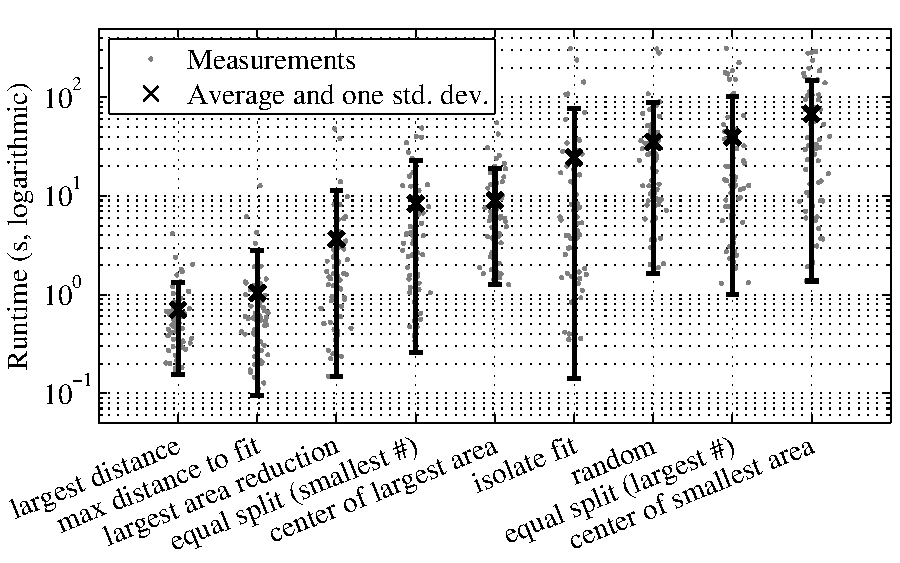
\includegraphics[width=0.95\linewidth]{images/typical_random_splitting_strategies.pdf}}
Different splitting strategies result in vastly different performance.
Note that  `split into equal sized problems' is one of the worst strategies for
branch and bound.
  }
%%%%%%%%%%%%%%%%%%%%%%%%%%%%%%%%%%%%%%%%%%%%%%%%%%%%%%%%%%%%%%%%%%%%%%%%%%%%%%
\headerbox{Solution}{name=solution,column=1,row=0,below=results,above=strategy}{
  %%%%%%%%%%%%%%%%%%%%%%%%%%%%%%%%%%%%%%%%%%%%%%%%%%%%%%%%%%%%%%%%%%%%%%%%%%%%%%
  This discrete optimization is solved by Branch and Bound, which is a method to minimize a function over a set. It requires us to (1) efficiently specify solution subsets, (2) determine a lower bound on the minimal cost of the solutions within a subset, and (3) specify a strategy to split a solution subset into two new subsets.
%\begin{enumerate}[itemsep=2pt,parsep=0pt]
%  \item Start with the set of all elements $\SET Q=\{ \AllSelections \}$
%  \item \textbf{Repeat}:
%  \begin{enumerate}[itemsep=2pt,parsep=0pt,topsep=2pt]
%  \item  Take the minimal subset\vspace{-0.7em}
%    \begin{align}
%      \J_i &\leftarrow \argmin_{\J_i \in \SET Q} g(\J_i)\\
%                  \SET Q   &\leftarrow \SET Q \setminus \{ \J_i \}\nonumber
%    \end{align}
%  \item
%    \textbf{Return} $\Selection$ \textbf{if} $\J_i=\{\Selection\}$ is a single element.
%  \item Split $\J_i$ into \vspace{-0.7em}
%    \begin{align}
%      \J_i^1 &\subset \J_i, \J_i^2 \subset \J_i\\\quad\text{ s.t. }\J_i &= \J_i^1 \cup \J_i^2.\nonumber
%    \end{align}
%  \item Add the new subsets to the candidates\vspace{-0.7em}
%    \begin{align}
%      \SET Q &\leftarrow \SET Q \cup \{ \J_i^1, \J_i^2 \}\nonumber
%    \end{align}
%  \end{enumerate}
%\end{enumerate}

  The ingredients in our case are:
 \begin{enumerate}
 \item Solution subsets are created by taking subsets of landmark
 candidates, and considering the Kartesian product of all selected landmark
 candidates
 \item We bound the cost for such a solution set by taking for each
 landmark the minimal distance to the convex hull of the selected candidates
% \begin{align}
%   g(\J) &= \min_{\Params} \sum_i \rho\left( d_{\text{convex hull}}(\l_i^{\J_i}, m_i(\Params)) \right)\\
%         &< \min_{\Params} \min %\nonumber\\
%   d_{\text{convex hull}}(\l_i^\J, \VEC x) &=  \min_{c \in \text{convex hull}(\l_i^{\J})}\normLR{ x - c }.
% \end{align}
 \item We found that splitting landmark candidates such that the convex hull of the resulting two landmark candidates are as distant as possible is most effective.
 \end{enumerate}
  }

\end{poster}

\end{document}

